\documentclass[letterpaper,12pt,oneside,final]{book}

%%
%%  Gabarit de mémoire de maîtrise ou thèse de doctorat.
%%  Template for dissertations and theses @ Polytechnique Montreal.

%%  Normalement, il n'est pas nécessaire de modifier ce document
%%  sauf pour établir le langage (français ou anglais) et pour changer les noms des 
%%  fichiers à inclure.
%%  Usually, this document needs to be modified only to set up the language (French or English) 
%%  and to change the names of the files to include.
%%
%%  Version: 2018-07-31
%%
%%  Accepte les caractères accentués dans le document (UTF-8).


\makeatletter
\def\bstctlcite{\@ifnextchar[{\@bstctlcite}{\@bstctlcite[@auxout]}}
\def\@bstctlcite[#1]#2{\@bsphack
 \@for\@citeb:=#2\do{%
   \edef\@citeb{\expandafter\@firstofone\@citeb}%
   \if@filesw\immediate\write\csname #1\endcsname{\string\citation{\@citeb}}\fi}%
 \@esphack}
\makeatother

% LA COMMANDE SUIVANTE ÉTABLIT LE LANGAGE DE LA THÈSE : CHOISIR french POUR UNE THÈSE EN FRANÇAIS
% THE NEXT COMMAND DETERMINES THE LANGUAGE OF THE THESIS: CHOOSE english FOR A THESIS IN ENGLISH
\newcommand\Langue{french}            

\usepackage{ifthen}
\usepackage[utf8]{inputenc}
%%
%% Support pour l'anglais et le français (français par défaut).
%\usepackage[cyr]{aeguill}
\usepackage{lmodern}      % Police de caractères plus complète et généralement indistinguable visuellement de la police standard de LaTeX (Computer Modern).
\usepackage[T1]{fontenc}  % Bon encodage des caractères pour qu'Acrobat Reader reconnaisse les accents et les ligatures telles que ffi.

% le langage par défaut est le dernier de la liste, c'est-à-dire français
\ifthenelse{\equal{\Langue}{english}}{
	\usepackage[frenchb,english]{babel}
}{
	\usepackage[english,frenchb]{babel} 
}

%%
%% Charge le module d'affichage graphique.
\usepackage{graphicx}
\usepackage{epstopdf}  % Permet d'utiliser des .eps avec pdfLaTeX.
%%
%% Recherche des images dans les répertoires.
\graphicspath{{./images/}{./dia/}{./gnuplot/}}
%%
%% Un float peut apparaître seulement après sa définition, jamais avant.
\usepackage{flafter,placeins}
%%
%% Utilisation de natbib pour les citations et la bibliographie.
%\usepackage{natbib}
%%
%% Autres packages.
\usepackage{amsmath,color,soulutf8,longtable,colortbl,setspace,xspace,url,pdflscape,cite}
%%
%% Support des acronymes.
\usepackage[nolist]{acronym}
\onehalfspacing                % Interligne 1.5.
%%
%% Définition d'un style de page avec seulement le numéro de page à
%% droite. On s'assure aussi que le style de page par défaut soit
%% d'afficher le numéro de page en haut à droite.
\usepackage{fancyhdr}
\fancypagestyle{pagenumber}{\fancyhf{}\fancyhead[R]{\thepage}}
\renewcommand\headrulewidth{0pt}
\makeatletter
\let\ps@plain=\ps@pagenumber
\makeatother
%%
%% Module qui permet la création des bookmarks dans un fichier PDF.
%\usepackage[dvipdfm]{hyperref}
\usepackage{hyperref}
\usepackage{caption}  % Hyperlien vers la figure plutôt que son titre.
\makeatletter
\providecommand*{\toclevel@compteur}{0}
\makeatother
%%
%% Définitions spécifiques au format de rédaction de Poly.
%% Here we define the Poly formatting.
\RequirePackage[\Langue]{MemoireThese}
%%
%% Définitions spécifiques à l'étudiant.
%!TEX root = ./Document.tex
%% -----------------------------------
%% ---> À MODIFIER PAR L'ETUDIANT / TO BE MODIFIED BY THE STUDENT <---
%% -----------------------------------
%%
%% Commandes qui affichent le titre du document, le nom de l'auteur, etc.
\newcommand\monTitre{Décodage de codes polaires sur des architectures programmables.}
\newcommand\monPrenom{Mathieu}
\newcommand\monNom{Léonardon}
\newcommand\monDepartement{Génie \'Electrique}  % Department
\newcommand\maDiscipline{\'Electronique}
\newcommand\monDiplome{D}        % (M)aîtrise ou (D)octorat / (M)aster or Ph(D)
\newcommand\anneeDepot{2018}    % Year
\newcommand\moisDepot{Novembre}       % Month
\newcommand\monSexe{M}           % "M" ou "F" = Gender
\newcommand\PageGarde{N}         % "O" ou "N" = Yes or No
\newcommand\AnnexesPresentes{O}  % "O" ou "N". Indique si le document comprend des annexes. / If the thesis includes annexes = O or N = No.
\newcommand\mesMotsClef{Codes polaires, Décodeur Logiciel, ASIP, Annulation Successive, Annulation Successive à Liste}
%%
%%  DEFINITION DU JURY
%%
%%  Pour la définition du jury, les macros suivantes sont definies:
%%  \PresidentJury, \DirecteurRecherche, \CoDirecteurRecherche, \MembreJury, \MembreExterneJury
%%
%%  Toutes les macros prennent 4 paramètres: Sexe (M/F), Prénom, Nom, Titres
\newcommand\monJury{\PresidentJury{M}{Mohamad}{Sawan}{Professeur Titulaire}\\
\DirecteurRecherche{M}{Yvon}{Savaria}{Professeur Titulaire}\\
\DirecteurRecherche{M}{Christophe}{J\'ego}{Professeur Titulaire}\\
\MembreJury{M}{Amer}{Baghdadi}{Professeur}\\
\MembreJury{M}{Emmanuel}{Casseau}{Professeur des Universités}\\
\MembreJury{M}{Camille}{Leroux}{Ma\^itre de Conf\'erences}\\
\MembreJury{M}{Olivier}{Muller}{Ma\^itre de Conf\'erences}\\
\MembreJury{M}{Charly}{Poulliat}{Professeur des Universités}}

\newcommand\templateVersion{EPM}

\ifthenelse{\equal{\monDiplome}{M}}{
\newcommand\monSujet{Mémoire de maîtrise}
\newcommand\monDipl{Maîtrise ès sciences appliquées}
}{
\newcommand\monSujet{Thèse de doctorat}
\newcommand\monDipl{Philosophi\ae{} Doctor}
}
%%
%% Informations qui sont stockées dans un fichier PDF.
\hypersetup{
  pdftitle={\monTitre},
  pdfsubject={\monSujet},
  pdfauthor={\monPrenom{} \monNom},
  pdfkeywords={\mesMotsClef},
  bookmarksnumbered,
  pdfstartview={FitV},
  hidelinks,
  linktoc=all
}

%!TEX root = ../my_thesis.tex

%%%%%%%%%%%%%%%%%%%%%%%%%%%%%%%%%%%%%%%%%%%%%%
%
%		Thesis Settings
%		Custom settings
%
%		2011
%
%%%%%%%%%%%%%%%%%%%%%%%%%%%%%%%%%%%%%%%%%%%%%%

%
%   Use this file for your own custom packages, command-definitions, etc...
%


% the following lines are for creating a simplified TO-DO box. However since boites is not per default installed with all latex-distributions, we have removed this example again
% if you want to use it and do not have "boites" installed, you can get it from here: http://www.ctan.org/tex-archive/macros/latex/contrib/boites
%
%\usepackage{boites,boites_exemples}
%\newcommand{\todolist}[1]{\begin{boiteepaisseavecuntitre}{TO DO in this chapter} #1 \end{boiteepaisseavecuntitre}}  % creates a little box
% %\newcommand{\todolist}[1]{}  % to be used when to do is not to be printed

\setcounter{secnumdepth}{4}

\usepackage[french]{minitoc} %rappel du plan du chapitre en cours
\renewcommand{\mtctitle}{}
\tightmtctrue
\nomtcrule
\renewcommand{\mtcSfont}{\small}

\newcommand{\minitocTITI}{\vspace*{1em}{\color{bleuUni}\hrule}\vspace*{-1ex}\minitoc\vspace*{-1ex}{\color{bleuUni}\hrule}%
}


%\usepackage{geometry} %pour la page de garde

\usepackage{tikz} %de même
\usetikzlibrary{shapes,arrows}
\usetikzlibrary{calc} 

\usepackage{array}
\usepackage{longtable} %pour la liste des notations

\usepackage[xindy]{glossaries}
\usepackage[toc,page]{appendix}
%\makeglossaries
%\makenoidxglossaries
\newacronym[longplural={Frames per Second}]{fpsLabel}{FPS}{Frame per Second}

\newglossaryentry{pi}
{
  name={\ensuremath{\pi}},
  description={ratio of circumference of circle to its
               diameter},
  sort=pi
}



\newacronym{lvm}{LVM}{Logical Volume Manager}



\usepackage{stmaryrd} % ll and rrbrackets
\usepackage{circuitikz}			% création d'images et de circuits électriques
\usepackage{pgfplots}				% package pour les graphiques
\usepackage{tikz-timing}			% package pour les chronogrammes
\usepackage{trig}				% fourni les fonctions trigonométriques

\usepackage{lettrine}
\pgfplotsset{compat=newest}

\usetikzlibrary{circuits, matrix, positioning}
% porte logique a plusieurs entrées
\usetikzlibrary{circuits.logic.CDH}
%\usetikzlibrary{circuits.ee.IEC}
\usepgfplotslibrary{groupplots}
\usepgfplotslibrary{colorbrewer}

\usepackage{pgffor}


\definecolor{Paired-2}{RGB}{166,206,227}
\definecolor{Paired-1}{RGB}{31,120,180}
\definecolor{Paired-4}{RGB}{178,223,138}
\definecolor{Paired-3}{RGB}{51,160,44}
\definecolor{Paired-6}{RGB}{251,154,153}
\definecolor{Paired-5}{RGB}{227,26,28}
\definecolor{Paired-8}{RGB}{253,191,111}
\definecolor{Paired-7}{RGB}{255,127,0}
\definecolor{Paired-10}{RGB}{202,178,214}
\definecolor{Paired-9}{RGB}{106,61,154}
\definecolor{Paired-12}{RGB}{255,255,153}
\definecolor{Paired-11}{RGB}{177,89,40}
\definecolor{Accent-1}{RGB}{127,201,127}
\definecolor{Accent-2}{RGB}{190,174,212}
\definecolor{Accent-3}{RGB}{253,192,134}
\definecolor{Accent-4}{RGB}{255,255,153}
\definecolor{Accent-5}{RGB}{56,108,176}
\definecolor{Accent-6}{RGB}{240,2,127}
\definecolor{Accent-7}{RGB}{191,91,23}
\definecolor{Accent-8}{RGB}{102,102,102}
\definecolor{Spectral-1}{RGB}{158,1,66}
\definecolor{Spectral-2}{RGB}{213,62,79}
\definecolor{Spectral-3}{RGB}{244,109,67}
\definecolor{Spectral-4}{RGB}{253,174,97}
\definecolor{Spectral-5}{RGB}{254,224,139}
\definecolor{Spectral-6}{RGB}{255,255,191}
\definecolor{Spectral-7}{RGB}{230,245,152}
\definecolor{Spectral-8}{RGB}{171,221,164}
\definecolor{Spectral-9}{RGB}{102,194,165}
\definecolor{Spectral-10}{RGB}{50,136,189}
\definecolor{Spectral-11}{RGB}{94,79,162}
\definecolor{Set1-1}{RGB}{228,26,28}
\definecolor{Set1-2}{RGB}{55,126,184}
\definecolor{Set1-3}{RGB}{77,175,74}
\definecolor{Set1-4}{RGB}{152,78,163}
\definecolor{Set1-5}{RGB}{255,127,0}
\definecolor{Set1-6}{RGB}{255,255,51}
\definecolor{Set1-7}{RGB}{166,86,40}
\definecolor{Set1-8}{RGB}{247,129,191}
\definecolor{Set1-9}{RGB}{153,153,153}
\definecolor{Set2-1}{RGB}{102,194,165}
\definecolor{Set2-2}{RGB}{252,141,98}
\definecolor{Set2-3}{RGB}{141,160,203}
\definecolor{Set2-4}{RGB}{231,138,195}
\definecolor{Set2-5}{RGB}{166,216,84}
\definecolor{Set2-6}{RGB}{255,217,47}
\definecolor{Set2-7}{RGB}{229,196,148}
\definecolor{Set2-8}{RGB}{179,179,179}
\definecolor{Dark2-1}{RGB}{27,158,119}
\definecolor{Dark2-2}{RGB}{217,95,2}
\definecolor{Dark2-3}{RGB}{117,112,179}
\definecolor{Dark2-4}{RGB}{231,41,138}
\definecolor{Dark2-5}{RGB}{102,166,30}
\definecolor{Dark2-6}{RGB}{230,171,2}
\definecolor{Dark2-7}{RGB}{166,118,29}
\definecolor{Dark2-8}{RGB}{102,102,102}
\definecolor{Reds-1}{RGB}{255,245,240}
\definecolor{Reds-2}{RGB}{254,224,210}
\definecolor{Reds-3}{RGB}{252,187,161}
\definecolor{Reds-4}{RGB}{252,146,114}
\definecolor{Reds-5}{RGB}{251,106,74}
\definecolor{Reds-6}{RGB}{239,59,44}
\definecolor{Reds-7}{RGB}{203,24,29}
\definecolor{Reds-8}{RGB}{165,15,21}
\definecolor{Reds-9}{RGB}{103,0,13}
\definecolor{Greens-1}{RGB}{247,252,245}
\definecolor{Greens-2}{RGB}{229,245,224}
\definecolor{Greens-3}{RGB}{199,233,192}
\definecolor{Greens-4}{RGB}{161,217,155}
\definecolor{Greens-5}{RGB}{116,196,118}
\definecolor{Greens-6}{RGB}{65,171,93}
\definecolor{Greens-7}{RGB}{35,139,69}
\definecolor{Greens-8}{RGB}{0,109,44}
\definecolor{Greens-9}{RGB}{0,68,27}
\definecolor{Blues-1}{RGB}{247,251,255}
\definecolor{Blues-2}{RGB}{222,235,247}
\definecolor{Blues-3}{RGB}{198,219,239}
\definecolor{Blues-4}{RGB}{158,202,225}
\definecolor{Blues-5}{RGB}{107,174,214}
\definecolor{Blues-6}{RGB}{66,146,198}
\definecolor{Blues-7}{RGB}{33,113,181}
\definecolor{Blues-8}{RGB}{8,81,156}
\definecolor{Blues-9}{RGB}{8,48,107}

\definecolor{falseframe}{RGB}{254,178,76}
\definecolor{correctframe}{RGB}{44,162,95}
\definecolor{falsebit}{RGB}{227,74,51}
\definecolor{correctbit}{RGB}{67,162,202}

\DeclareMathOperator{\card}{card}
\DeclareMathOperator*{\maxstar}{max*}
\DeclareMathOperator*{\argmax}{arg\,max}
\DeclareMathOperator*{\decide}{decide}

%\let\emph\relax % there's no \RedeclareTextFontCommand
%\DeclareTextFontCommand{\emph}{\bfseries\em}
\usetikzlibrary{patterns}

\usepackage{version}
\usepackage[export]{adjustbox}
\reversemarginpar

\newcommand{\e}{\mathrm{e}}
\usepackage{multirow}

\usepackage{arydshln}
\usepackage{bm}

\makeatletter
\def\adl@drawiv#1#2#3{%
        \hskip.5\tabcolsep
        \xleaders#3{#2.5\@tempdimb #1{1}#2.5\@tempdimb}%
                #2\z@ plus1fil minus1fil\relax
        \hskip.5\tabcolsep}
\newcommand{\cdashlinelr}[1]{%
  \noalign{\vskip\aboverulesep
           \global\let\@dashdrawstore\adl@draw
           \global\let\adl@draw\adl@drawiv}
  \cdashline{#1}
  \noalign{\global\let\adl@draw\@dashdrawstore
           \vskip\belowrulesep}}
\makeatother

\usepackage{scalerel}

\def\thumbsup{\includegraphics[width=15pt]{head/down.png}}
\def\thumbsdown{\includegraphics[width=15pt]{head/up.png}}
\def\thumbsmid{\includegraphics[width=15pt]{head/mid.png}}

\usepackage[french,onelanguage, ruled, linesnumbered, vlined]{algorithm2e}
\SetAlFnt{\small}
\usepackage{multibib}
\newcites{mine}{Publications}

\DecimalMathComma

\newcommand\ddfrac[2]{\frac{\displaystyle #1}{\displaystyle #2}}

\makeatletter
\AtBeginDocument{\let\book@l@chapter\l@chapter}
\newcommand{\demotechaptersintoc}{%
  \addtocontents{toc}{\let\protect\l@chapter\protect\l@section}%
}
\newcommand{\promotechaptersintoc}{%
  \addtocontents{toc}{\let\protect\l@chapter\protect\book@l@chapter}%
}
\newcommand{\mb}[1]{\mathbold{#1}}
  % place your custom packages, etc... in this file!
\usepackage{eulervm}
\usepackage{amsfonts}
\usepackage{subfig}
%%
%% Il y a un document par chapitre du mémoire.
%%
\definecolor{bleuUni}{RGB}{0, 157, 224}

\begin{document}
\bstctlcite{IEEEexample:BSTcontrol}

%%
%% Page de titre du mémoire.
\frontmatter
% Compte optionellement la pazge de garde dans la pagination.
\ifthenelse{\equal{\PageGarde}{O}}{\addtocounter{page}{1}}{}
\thispagestyle{empty}%
\begin{center}%
\vspace*{\stretch{1}}
UNIVERSITÉ DE MONTRÉAL\\
\vspace*{\stretch{1}}
\MakeUppercase{\monTitre}\\
\vspace*{\stretch{1}}
\MakeUppercase{\monPrenom~\monNom}\\
DÉPARTEMENT DE \MakeUppercase{\monDepartement}\\
ÉCOLE POLYTECHNIQUE DE MONTRÉAL\\
\vspace*{\stretch{1}}
\ifthenelse{\equal{\monDiplome}{M}}{MÉMOIRE PRÉSENTÉ}{THÈSE PRÉSENTÉE} EN VUE DE L'OBTENTION\\
DU DIPLÔME DE \MakeUppercase{\monDipl}\\
(\MakeUppercase{\maDiscipline})\\
\MakeUppercase{\moisDepot} \anneeDepot
\end{center}%
\vspace*{\stretch{1}}
\copyright~\monPrenom~\monNom, \anneeDepot.
%%
%% Identification des membres du jury.
%%
\newpage\thispagestyle{empty}%
\begin{center}%
\vspace*{\stretch{2}}
\ul{UNIVERSITÉ DE MONTRÉAL}\\
\vspace*{\stretch{1}}
\ul{ÉCOLE POLYTECHNIQUE DE MONTRÉAL}\\
\vspace*{\stretch{2}}
Ce\ifthenelse{\equal{\monDiplome}{M}}{~mémoire intitulé}{tte thèse intitulée}:\\
\vspace*{\stretch{1}}
\MakeUppercase{\monTitre}\\
\vspace*{\stretch{2}}
\end{center}%
\begin{flushleft}
présenté\ifthenelse{\equal{\monDiplome}{M}}{}{e}
par:~\ul{\mbox{\MakeUppercase{\monNom} \monPrenom}}\\
en vue de l'obtention du diplôme de:~\ul{\mbox{\monDipl}}\\
a été dûment accepté\ifthenelse{\equal{\monDiplome}{M}}{}{e} par le jury d'examen constitué de:\end{flushleft}
\vspace*{\stretch{2}}
\monJury
%%
\pagestyle{pagenumber}%
\cleardoublepage
\thispagestyle{empty}

\vspace*{\fill}

\begin{raggedleft}
A mes parents, à ma compagne.\\
\end{raggedleft}
\vspace*{\fill}

          % Dédicace du document.
%!TEX root = ../my_thesis.tex
%\cleardoublepage
\addcontentsline{toc}{chapter}{Remerciements}
\chapter*{Remerciements}
%\markboth{Résumé}{Résumé}
% put your text here
%\vskip1em

Je tiens en premier lieu à remercier les membres du jury pour l'intérêt qu'ils ont porté à ces travaux. Je remercie donc 
très chaleureusement Monsieur Jean-Pierre \bsc{Cances}, professeur de l'Université de Limoges et Monsieur Michel 
\bsc{Jézéquel}, professeur de l'Institut Mines-Télecom Atlantique de m'avoir fait l'honneur de rapporter ce travail de thèse.
Je remercie vivement Monsieur Charly \bsc{Poulliat}, professeur de l'Institut National Polytechnique de Toulouse 
d'avoir présidé le jury.

% Je souhaite également expressément remercier les différentes personnes ayant relu le manuscrit et contribué à cette 
% version finale.

Merci à Messieurs Benjamin \bsc{Gadat} et Nicolas \bsc{Van Wambeke} pour nos échanges et vos encadrements
dans le cadre de vos fonctions respectives au sein de Thales Alenia Space.

Je remercie grandement Bertrand, Camille et Christophe qui ont su répondre à mes (trop ?) nombreuses sollicitations durant
ces années.\\
Bertrand, merci pour ton soutien sans faille et ton dynamisme quotidien exemplaire, j'ai particulièrement apprécié travailler
à tes côtés. \\
Camille, merci pour l'ensemble de nos moments passés ensemble; que ce soit au sein du laboratoire, lors de nos 
enseignements matinaux ou enfin en dehors de tout ceci.\\
Christophe, merci d'avoir toujours fait en sorte de mettre en place le cadre de travail le plus agréable possible, merci 
pour tes relectures en première ligne et ton animation d'équipe de haut-vol.

Merci à tous mes collègues d'avoir contribué à l'excellente ambiance de travail. Tout d'abord, l'ensemble de l'équipe CSN
et plus généralement les membres du groupe Conception. Ainsi, merci Jérémie, Dominique, Jean-Baptiste, Adrien, Camilo, 
Guillaume B., Guillaume D., Imen, Jonathan, Mathieu, Olivier, Vincent, Yann.  Merci aussi à François, Nathalie et Yann.
Enfin, un grand merci à Raphaël, sans qui ces années au laboratoire auraient été fondamentalement différentes.\\
Au niveau du groupe Signal et Image, merci à Guillaume F. et à Romain pour nos nombreux échanges.

Je tiens à remercier tout particulièrement Arnaud pour m'avoir fait découvrir le monde de la recherche, sans qui il ne me serait
venu l'envie de réaliser une thèse.

Finalement, je remercie amoureusement Fanny qui a su me supporter et tolérer des horaires de retour bien trop tardifs 
ainsi qu'une disponibilité dans notre vie commune bien trop faible.
     % Remerciements.
%!TEX root = ../my_thesis.tex
%\cleardoublepage
\addcontentsline{toc}{chapter}{Résumés}
\chapter*{Résumé}
%\markboth{Résumé}{Résumé}
% put your text here
\vskip1em


Les codes polaires constituent une classe de codes correcteurs d'erreurs inventés récemment qui suscite l'intérêt des chercheurs et des industriels, comme en atteste leur sélection pour le codage des canaux de contrôle dans la prochaine génération de téléphonie mobile (5G). Un des enjeux des futurs réseaux mobiles est la virtualisation des traitements numériques du signal, et en particulier les algorithmes de codage et de décodage.  Afin d'améliorer la flexibilité du réseau, ces algorithmes doivent être décrits de manière logicielle et être déployés sur des architectures programmables. Une telle infrastructure  de réseau permet de mieux répartir l'effort de calcul sur l'ensemble des \noeuds et d'améliorer la coopération entre cellules. Ces techniques ont pour but de réduire la consommation d'énergie, d'augmenter le débit et de diminuer la latence des communications. Les travaux présentés dans ce manuscrit portent sur l'implémentation logicielle des algorithmes de décodage de codes polaires et la conception d'architectures programmables spécialisées pour leur exécution.

Une des caractéristiques principales d'une chaîne de communication mobile est l'instabilité du canal de communication. Afin de remédier à cette instabilité, des techniques de modulations et de codages adaptatifs sont utilisées dans les normes de communication. Ces techniques impliquent que les décodeurs supportent une vaste gamme de codes : ils doivent être génériques. La première contribution de ces travaux est l'implémentation logicielle de décodeurs génériques des algorithmes de décodage "à Liste" sur des processeurs à usage général. En plus d'être génériques, les décodeurs proposés sont également flexibles. Ils permettent en effet des compromis entre pouvoir de correction, débit et latence de décodage par la paramétrisation fine des algorithmes. En outre, les débits des décodeurs proposés atteignent les performances de l'état de l'art et, dans certains cas, les dépassent.

La deuxième contribution de ces travaux est la proposition d'une nouvelle architecture programmable performante spécialisée dans le décodage de codes polaires. Elle fait partie de la famille des processeurs à jeu d'instructions dédiés à l'application. Un processeur de type RISC à faible consommation en constitue la base. Cette base est ensuite configurée, son jeu d'instructions est étendu et des unités matérielles dédiées lui sont ajoutées. Les simulations montrent que cette architecture atteint des débits et des latences proches des implémentations logicielles de l'état de l'art sur des processeurs à usage général. La consommation énergétique est réduite d'un ordre de grandeur. En effet, lorsque l'on considère le décodage par annulation successive d'un code polaire (1024,512), l'énergie nécessaire par bit décodé est de l'ordre de 10 nJ sur des processeurs à usage général contre 1 nJ sur les processeurs proposés.

La troisième contribution de ces travaux est également une architecture de processeur à jeu d'instructions dédié à l'application. Elle se différencie de la précédente par l'utilisation d'une méthodologie de conception alternative. Au lieu d'être basée sur une architecture de type RISC, l'architecture du processeur proposé fait partie de la classe des architectures déclenchées par le transport. Elle est caractérisée par une plus grande modularité qui permet d'améliorer très significativement l'efficacité du processeur. Les débits mesurés sont alors supérieurs à ceux obtenus sur les processeurs à usage général. La consommation énergétique est réduite à environ 0.1 nJ par bit décodé pour un code polaire (1024,512) avec l'algorithme de décodage par annulation successive. Cela correspond à une réduction de deux ordres de grandeur en comparaison de la consommation mesurée sur des processeurs à usage général.
 
\vskip0.5cm
\emph{Mots clefs :} Codes polaires, Décodeur Logiciel, ASIP, Annulation Successive, Annulation Successive à Liste
\cleardoublepage
\chapter*{Abstract}
\vskip1em

Polar codes are a recently invented class of error-correcting codes that are of interest to both researchers and industry, as evidenced by their selection for the coding of control channels in the next generation of cellular mobile communications (5G). One of the challenges of future mobile networks is the virtualization of digital signal processing, including channel encoding and decoding algorithms. In order to improve network flexibility, these algorithms must be written in software and deployed on programmable architectures. Such a network infrastructure allow dynamic balancing of the computational effort across the network, as well as inter-cell cooperation. These techniques are designed to reduce energy consumption, increase throughput and reduce communication latency. The work presented in this manuscript focuses on the software implementation of polar codes decoding algorithms and the design of programmable architectures specialized in their execution.

One of the main characteristics of a mobile communication chain is that the state of communication channel changes over time. In order to address issue, adaptive modulation and coding techniques are used in communication standards. These techniques require the decoders to support a wide range of codes: they must be generic. The first contribution of this work is the software implementation of generic decoders for "List" polar decoding algorithms on general purpose processors. In addition to their genericity, the proposed decoders are also flexible. Trade-offs between correction power, throughput and decoding latency are enabled by fine-tuning the algorithms. In addition, the throughputs of the proposed decoders achieve state-of-the-art performance and, in some cases, exceed it.

The second contribution of this work is the proposal of a new high-performance programmable architecture specialized in polar code decoding. It is part of the family of Application Specific Instruction-set Processors (ASIP). The base architecture is a RISC processor. This base architecture is then configured, its instruction set is extended and dedicated hardware units are added. Simulations show that this architecture achieves throughputs and latencies close to state-of-the-art software implementations on general purpose processors. Energy consumption is reduced by an order of magnitude. The energy required per decoded bit is about 10 nJ on general purpose processors compared to 1 nJ on proposed processors when considering the Successive Cancellation (SC) decoding algorithm of a polar code (1024,512).

The third contribution of this work is also the design of an ASIP architecture. It differs from the previous one by the use of an alternative design methodology. Instead of being based on a RISC architecture, the proposed processor architecture is part of the class of Transport Triggered Architectures (TTA). It is characterized by a greater modularity that allows to significantly improve the efficiency of the processor. The measured flow rates are then higher than those obtained on general purpose processors. The energy consumption is reduced to about 0.1 nJ per decoded bit for a polar code (1024,512) with the SC decoding algorithm. This corresponds to a reduction of two orders of magnitude compared to the consumption measured on general purpose processors.

\vskip0.5cm
\emph{Key words:} Polar-codes...
      % Résumé du sujet en français.

{\setlength{\parskip}{0pt}
%%
%% Table des matières.
\ifthenelse{\equal{\Langue}{english}}{
	\renewcommand\contentsname{TABLE OF CONTENTS}
}{
	\renewcommand\contentsname{TABLE DES MATIÈRES}
}
\tableofcontents
%%
%% Liste des tableaux.
\ifthenelse{\equal{\Langue}{english}}{
	\renewcommand\listtablename{LIST OF TABLES}
}{
	\renewcommand\listtablename{LISTE DES TABLEAUX}
}\listoftables
%%
%% Table des figures.
\ifthenelse{\equal{\Langue}{english}}{
	\renewcommand\listfigurename{LIST OF FIGURES}
}{
	\renewcommand\listfigurename{LISTE DES FIGURES}
}\listoffigures
%%
%% Liste des annexes au besoin.
}

%!TEX root = ../my_thesis.tex
\chapter*{Liste des notations}
\markboth{Liste des notations}{Liste des notations}
\addcontentsline{toc}{chapter}{Liste des notations}
% put your text here
\begin{center}

\begin{longtable}{ p{.18\textwidth}  p{.82\textwidth} } 

$C$						& 	Capacité du canal de transmission														\\
$\mathbb{E}$            &   Espérance mathématique                                                                  \\
$E_b$         	 		&	Énergie moyenne par bit d'information     												\\
$\text{erfc}(\cdot)$    &	Fonction d'erreur complémentaire     													\\
$\text{sgn}(\cdot)$    	&	Fonction signe																			\\
$\mathbf{c}$			& 	Mot de code 																			\\
$\mathbf{\hat{d}}$		&	Mot décidé																				\\
$R$     	 			&	Rendement du code ($R=K/N$)       														\\
$K$     	  			&	Taille du mot d'information non codé     												\\
$N$     	 			& 	Taille du mot de code                													\\
$L(\cdot)$				&	Valeur LLR 																				\\
$\sigma$				&   Variance du bruit																		\\


		
\end{longtable}

\end{center}
\chapter*{Liste des acronymes}
\markboth{Liste des acronymes}{Liste des acronymes}
\addcontentsline{toc}{chapter}{Liste des acronymes}
% put your text here
\begin{center}

\begin{longtable}{ p{.18\textwidth}  p{.82\textwidth} } 

5G        & 5th generation of cellular mobile communications       \\
ARM       & Advanced Risc Machine                                  \\
ASIC      & Application Specific Integrated Circuit                \\
ASIP      & Application Specific Instruction set Computer          \\
AWGN      & Additive White Gaussian Noise                          \\
BI-AWGNC  & Binary Input - AWGN Channel                            \\
% BE      & Bit Error, nombre d'erreurs binaires                   \\
BER       & Bit Error Rate                                         \\
BP        & Belief Propagation                                     \\
BPSK      & Binary Phase-Shift Keying                              \\
CASCL     & CRC-Aided Successive Cancellation List                 \\
CRC       & Cyclic Redundancy Check                                \\
% FE      & Frame Error                                            \\
FASCL     & Fully Adaptive Successive Cancellation List            \\
FER       & Frame Error Rate                                       \\
FPGA      & Field Programmable Gate Array                          \\
FLIX      & Flexible Length Instruction Extensions                 \\
% LDPC    & Low Density Parity Check Codes                         \\
LLR       & Log Likelihood Ratio                                   \\
LSU       & Load / Store Unit                                      \\
MIPP      & My Intrinsics Plus Plus library                        \\
PASCL     & Partially Adaptive Successive Cancellation List        \\
PE        & Processing Element                                     \\
PS        & Partial Sum                                            \\
PU        & Processing Unit                                        \\
RISC      & Reduced Instruction Set Computer                       \\
SC        & Successive Cancellation                                \\
SCAN      & Soft CANcellation                                      \\
SCF       & Successive Cancellation Flip                           \\
SCL       & Successive Cancellation List                           \\
SCS       & Successive Cancellation Stack                          \\
SNR       & Signal-to-Noise Ratio                                  \\
SPC       & Single Parity Check                                    \\
REP       & REPetition                                             \\
TCE       & TTA Co-design Environment                              \\
TTA       & Transport Triggered Architecture                       \\
\end{longtable}

\end{center}
%\vspace*{\fill}

       % Liste des sigles et abréviations.
\ifthenelse{\equal{\AnnexesPresentes}{O}}{\listofappendices}{}
\mainmatter
%!TEX root = ../my_thesis.tex
\chapter*{Introduction}
\markboth{Introduction}{Introduction}
\addcontentsline{toc}{chapter}{Introduction}

Les travaux développés dans le cadre de cette thèse portent sur la proposition de méthodes et la définition 
d'architectures associées permettant 
l'amélioration des performances de décodage des turbo codes. Tout d'abord, le contexte des codes correcteurs d'erreurs 
est dressé. Ceci mène à la problématique traitée tout au long de ce manuscrit. L'agencement du manuscrit est 
ensuite détaillé. Enfin, les contributions réalisées au cours des travaux de thèse sont énoncés.

\section*{Contexte et problématique}
L'année 2016 marque le centenaire de la naissance de Claude Shannon. Ingénieur en génie électrique et mathématicien, il 
est le père de la théorie de l'information. L'origine de cette discipline -- se plaçant à l'intersection des mathématiques, 
des statistiques, du traitement du signal et de l'électronique -- remonte à la publication de l'article fondateur 
"A mathematical Theory of Communication" \cite{shannon_mathematical_2001}, paru en 1948 dans la revue interne des laboratoires Bell. Quelques mois 
auparavant, au même endroit, le transistor est inventé par John Bardeen, Walter Brattain et William Shockley. Ces deux 
avancées scientifiques, concomitantes, ont en moins de 70 ans amplement modifié nos sociétés et leurs manières d’interagir entre elles. 
% En effet, d'une part, ce semi-conducteur permet de représenter par son état de conduction (ouvert ou fermé) les deux états d'une
% information binaire. D'autre part l'unité de mesure de l'apport de d'une information, le bit, correspond à cette levée 
% d'incertitude lors de la réponse vrai ou faux.

Via la formalisation de l'information de manière abstraite et mathématique, le sens d'un message n'importe plus. Il est 
désormais possible de mesurer et de quantifier l'information. %En découle la possibilité de théoriser la 
Dans son article, Shannon montre que chaque canal de transmission peut faire transiter une quantité maximale 
d'information de manière fiable. De fait, en raison du bruit inhérent aux canaux de transmission, des erreurs peuvent apparaître
lors de la réception du message. Afin de palier cela, Shannon démontre qu'il existe un système de codage correcteur d'erreurs, 
%basé sur l'insertion d'informations redondantes à l’émission, 
basé sur l'envoi d'informations redondantes
permettant lors de la réception de corriger complètement les effets des distorsions et ainsi, de reconstituer parfaitement
le contenu du message émis. Cependant, Shannon ne fournit aucune indication quant à la façon de concevoir un tel code
correcteur d'erreurs.

Face à l'enjeu que représente la transmission fiable de l'information, la communauté scientifique s'est consacrée à la 
construction de tels codes. Tout d'abord, en 1950, Richard Hamming invente un code éponyme permettant de corriger tous 
les messages contenant une unique erreur binaire \cite{hamming}. S'en est suivi quinze années de découvertes successives avec les codes de Reed-Muller \cite{reedmuller1,reedmuller2} en 1954,
puis les codes convolutifs par Peter Elias en 1955 \cite{elias}, les codes de BCH en 1959 \cite{hocquenghem1959codes,bose1960class}, les codes LDPC par Robert Gallager en 1962 \cite{gallager1962low}.
Ces différentes familles de codes correcteurs d'erreurs permettent de corriger de 1 à $n$ erreurs de transmission dans un message en fonction de la quantité d'information redondante ajoutée lors de l'émission du message.
Enfin, en 1966, David Forney introduit le principe de la concaténation de codes correcteurs d'erreurs \cite{forney1966concatenated}. Cependant, à partir de 1966, les avancées
sur la construction de codes correcteurs d'erreurs se font rares. Cela fait alors dire à Robert McEliece en 1971 que 
\og Le codage de canal est mort \fg\cite{codingdead}. 

C'était sans compter sur la découverte deux décennies plus tard des turbo codes par Claude Berrou et Alain Glavieux \cite{berrouTC}. 
Grâce à leurs performances, cette nouvelle famille de codes correcteurs d'erreurs se place en rupture avec les
schémas de codage alors existants. Dès leur introduction, les turbo codes sont employés dans différents 
standards de communications numériques adressant des contextes applicatifs divers et variés. L'une des métriques de 
performance d'un code correcteur d'erreurs est sa capacité de correction en fonction de la qualité de transmission. 
Pour un turbo code et d'autres familles de codes correcteurs d'erreurs, une telle courbe de performance est divisée en deux parties. Dans la première, nommée région de 
convergence, un faible incrément de la qualité de transmission résulte en une amélioration importante des performances de
décodage. En revanche, dans la région du plancher d'erreurs, l'augmentation de la qualité de transmission ne résulte qu'en
une amélioration marginale des performances de décodage. Cette région est alors particulièrement limitante pour des applications
nécessitant de très faibles taux d'erreurs.

Par exemple, 
pour le stockage de masse, les taux d'erreurs cibles sont de plus en plus critiques et atteignent actuellement $10^{-18}$.
Dans un contexte de 
lien optique en espace libre, correspondant à des communications satellitaires par faisceau optique, un 
plancher d'erreurs situé sous les $10^{-9}$ est recherché. Le même ordre de grandeur est attendu pour le standard 
CCSDS-2. Enfin les applications de télémesure ou de 
contrôle-commande d'aéronef sans humain à bord nécessitent elles aussi des taux d'erreurs particulièrement faibles. Dès 
lors, une amélioration des performances de décodage, et notamment la réduction du plancher d'erreurs est primordiale.

D'autre part, lorsqu'un turbo code est retenu pour un standard de communications numériques, ses performances sont adaptées aux
contraintes applicatives correspondant au cas d'emploi de ce standard. Cependant, les besoins applicatifs évoluent au cours du temps et peuvent diverger de ceux originellement considérés. Ainsi, des exigences de plus faibles taux 
d'erreurs pour une qualité de transmission constante peuvent apparaître. Deux solutions sont alors envisageables. La première
consiste à repenser le code correcteur d'erreurs afin d'atteindre ces nouveaux besoins. Néanmoins, cette approche est 
particulièrement coûteuse. De fait, l'ensemble de l’infrastructure devient obsolète et un nouveau déploiement 
d'équipements, que ce soit pour la transmission ou la réception, s'avère nécessaire. Cette solution est par exemple 
difficilement envisageable pour un contexte de communications satellitaires.

Une autre solution consiste à modifier uniquement la partie réception. Dans ce contexte, les modifications des performances 
se situent au niveau des fonctions de réception. Ainsi, ces dernières années, la communauté scientifique a proposé différentes 
approches permettant d'améliorer les performances de décodage des turbo codes. Néanmoins, ces approches sont coûteuses
à mettre en œuvre. C'est pourquoi les implémentations matérielles de telles solutions sont rares. Les travaux conduits 
durant cette thèse répondent alors à la problématique de proposer de nouveaux algorithmes de décodage des
turbo codes. Ceux-ci doivent permettre une amélioration des performances de décodage tout en limitant le surcoût de l'implémentation matérielle 
des solutions de décodage mises en œuvre.
 La réponse à cette problématique, qui constitue le travail de thèse, est récapitulée dans ce manuscrit. Ce dernier est organisé 
 en quatre chapitres.

\section*{Structure du manuscrit de thèse}
Le premier chapitre expose les concepts et les notions associées aux travaux de thèse. Dans un premier temps, les notions 
essentielles des codes correcteurs d'erreurs sont abordées. Celles-ci sont illustrées par le théorème du codage de 
canal, une présentation des différentes familles de codes correcteurs d'erreurs et enfin des métriques permettant la 
caractérisation des performances de décodage d'un code correcteur d'erreurs. Dans un second temps, les turbo codes sont détaillés.
La construction des turbo codes est tout d'abord exposée. Dans un second temps, le principe de turbo décodage est expliqué. Ceci amène 
l'introduction de la problématique du plancher d'erreurs. Les raisons de son 
apparition ainsi que les propositions de la littérature quant à sa réduction sont alors détaillées.

Le deuxième chapitre est consacré à l'étude des oscillations de métriques impliquées dans le décodage itératif des 
turbo codes. Suite à une observation fine de celles-ci, un algorithme les exploitant est proposé. Celui-ci, inspiré 
d'une approche originellement développée pour les codes LDPC, permet d'améliorer les performances de décodage de turbo codes dans la 
zone de convergence. Cependant, ces améliorations ne sont pas observées pour toutes les familles de turbo codes. 
Finalement, une tentative d'utilisation des oscillations est considérée dans un contexte de décodage répété d'une même 
trame.

Le troisième chapitre traite de la contribution majeure de ces travaux de thèse. Elle consiste en la présentation d'une méthode 
permettant de corriger les erreurs résiduelles rencontrées dans la zone du plancher d'erreurs lors du décodage de turbo 
codes. À la faveur d'une prédiction analytique, les erreurs résiduelles sont caractérisées. Ceci permet alors la 
comparaison de différentes métriques permettant de les détecter. Une de ces métriques, grâce à son fort pouvoir 
d'identification, est alors retenue comme cœur de la proposition d'un algorithme de correction des erreurs résiduelles. 
Cet algorithme a pour propriété d'abaisser drastiquement le plancher d'erreurs de tous les turbo codes standardisés
qui ont pu être considérés dans ce manuscrit. 

Le quatrième chapitre est dédié à la description d'une architecture matérielle adaptée à l'algorithme de correction 
des erreurs résiduelles. Cet algorithme, par son principe, peut être vu comme une extension d'un turbo décodeur. Dès 
lors les différents ordonnancements de turbo décodage sont successivement présentés. Suite à cela, afin d'assurer la maîtrise de la complexité 
calculatoire de cet algorithme, une étude des différents paramètres 
sur les performances de décodages est menée. Celle-ci permet alors la proposition d'une architecture 
matérielle de référence adaptée à un ordonnancement particulier de turbo décodage. Le coût matériel de l'architecture 
est comparé à celui d'une architecture matérielle de turbo décodage équivalente. Finalement, des projections sont 
esquissées quant aux modifications requises à l'adaptation de cette architecture aux autres ordonnancements de turbo 
décodage existants.

\section*{Contributions des travaux de thèse}
Les différentes contributions originales de ces travaux de thèse sont : 
\begin{enumerate}
	\item La proposition d'un algorithme de décodage permettant l'amélioration de la convergence de décodage de 
	turbo codes dans certains contextes. Son principe est d'annuler la contribution des décodeurs élémentaires du 
	turbo décodeur lorsqu'un changement de signe sur cette contribution est détectée d'une itération à l'autre. Dans le
	cadre du standard CCSDS, des gains de $0,1$ dB sont observés en comparaison d'un turbo décodage conventionnel.
	Ceci est détaillé dans le deuxième chapitre.
	\item La proposition d'un algorithme de décodage basé sur le décodage successif d'une même trame permettant une 
	réduction limitée du plancher d'erreurs. Un abaissement d'un ordre de grandeur pour de hautes valeurs du rapport signal à bruit est atteint pour différents turbo codes. Cependant les gains sont obtenus au prix d'un surcoût calculatoire important. Ceci est détaillé dans le deuxième chapitre.
	\item La formalisation d'une prédiction de la distribution des erreurs résiduelles dans la zone du plancher 
	d'erreurs des turbo codes. Celle-ci se base directement sur le spectre de distances des turbo codes. Le spectre est
	plus 
	facile à obtenir que les fonctions recenseuses de poids jusqu'alors utilisées. Ceci est détaillé dans le troisième chapitre.
	\item La proposition d'un algorithme de décodage permettant une réduction drastique du plancher d'erreurs des 
	turbo codes standardisés grâce à la correction des erreurs résiduelles. Cet algorithme, nommé \textit{Flip and Check} a un surcoût en 
	terme de complexité calculatoire maîtrisé. Il permet d'abaisser le plancher d'erreurs d'au moins un ordre de grandeur 
	dans tous les contextes applicatifs considérés dans ce manuscrit. Ceci est détaillé dans le troisième chapitre.
	\item La proposition d'une architecture matérielle adaptée à l'algorithme Flip and Check de correction des erreurs résiduelles.
	Cette architecture matérielle démontre la possible intégration de la technique proposée pour des systèmes contraints, 
	grâce à un impact limité au niveau de la complexité calculatoire. De plus, la latence du 
	processus de turbo décodage n'est pas impactée. Ceci est détaillé dans le quatrième chapitre.\\
\end{enumerate}
Ces différentes contributions ont fait l'objet de publications scientifiques : \\
\begin{itemize}
	\item Communications nationales avec actes :
	\begin{itemize}
     	\item T. Tonnellier, C. Leroux, B. L. Gal, C. Jego, B. Gadat, and C. Poulliat,
		“L’algorithme Self-Corrected Max-Log-MAP pour le décodage des Turbo Codes”,
		18ème Journées Nationales du Réseau Doctoral en Micro-nanoélectronique (JNRDM), Bordeaux, 5-7 Mai, 2015.
		\item T. Tonnellier, C. Leroux, B. L. Gal, C. Jego, B. Gadat, and C. Poulliat, “Extension
		du principe self-corrected de l’information extrinsèque au décodage itératif de turbo
		codes,” in GRETSI, Sept 2015.
		\item T. Tonnellier, C. Leroux, B. L. Gal, C. Jego, B. Gadat, and N. V. Wambeke,“Correction 
		des erreurs résiduelles lors du processus de turbo décodage : algorithme et architecture,”
		in GDR Soc-SiP, June 2017.\\
	\end{itemize}
	\item Communications internationales avec actes :
	\begin{itemize}
		\item T. Tonnellier, C. Leroux, B. L. Gal, C. Jego, B. Gadat, and N. V. Wambeke,
		“Lowering the error floor of double-binary turbo codes : the Flip and Check algorithm”
		in 9th International Symposium on Turbo Codes and Iterative Information
		Processing (ISTC), Sept 2016, pp. 156–160.
		\item A. Cassagne, T. Tonnellier, C. Leroux, B. L. Gal, O. Aumage, and D. Barthou,
		“Beyond gbps turbo decoder on multi-core cpus,” in 9th International Sympo-
		sium on Turbo Codes and Iterative Information Processing (ISTC), Sept 2016, pp. 136–140.
		\item T. Tonnellier, C. Leroux, B. L. Gal, C. Jego, B. Gadat, and N. V. Wambeke,
		“Hardware architecture for lowering the error floor of lte turbo codes,” in 
		Conference on Design and Architectures for Signal and Image Processing (DASIP),
		Oct 2016, pp. 107–112.\\
	\end{itemize}
	\item Communication dans une revue internationale avec comité de lecture :
	\begin{itemize}
		\item T. Tonnellier, C. Leroux, B. L. Gal, B. Gadat, C. Jego, and N. V. Wambeke,
		“Lowering the error floor of turbo codes with CRC verification,” IEEE Wireless
		Communications Letters, vol. 5, no. 4, pp. 404–407, Aug 2016.
	\end{itemize}
\end{itemize}


% Les codes correcteurs d'erreurs sont une des solutions permettant d'améliorer la qualité des communications 
% numériques. Leur principe est d'introduire de la redondance dans la séquence d'information binaire afin de corriger 
% les erreurs de transmission durant la réception de l’information. Les turbo codes sont une des familles de codes 
% correcteurs d'erreurs parmi les plus performantes. Ils sont donc employés dans différents standards de communications
% numériques adressant des contextes applicatifs divers et variés. L'une des métriques de performance d'un code 
% correcteur d'erreurs est sa capacité de correction en fonction de la qualité de transmission. La région du plancher 
% d'erreur, inhérente à tout turbo décodage, est particulièrement limitante lors d'une nécessité de très faibles taux 
% d'erreurs.

% Lorsqu'un turbo code est choisi pour un standard de communications numérique, ses performances sont adaptées aux
% contraintes applicatives correspondant au cas d'emploi de ce standard. Cependant, les besoins applicatifs peuvent 
% évoluer au cours du temps et diverger de ceux originellement considérés. Ainsi, des exigences de plus faibles taux 
% d'erreur à qualité de transmission égale peuvent être nécessaires. Deux solutions sont alors envisageables. La première
% consiste à repenser le code correcteur d'erreur afin d'atteindre ces nouveaux besoins. Néanmoins, cette approche est 
% particulièrement coûteuse. De fait, l'ensemble de l’infrastructure est rendue obsolète et un nouveau déploiement 
% d'équipements, que ce soit pour la transmission ou la réception, devient nécessaire. Cette solution est par exemple 
% difficilement envisageable pour un contexte de communications satellitaires.

% Une autre solution consiste à modifier uniquement la partie réception. Dans ce cas, les modifications des performances 
% se situent au niveau du turbo décodeur. Ces dernières années, la communauté scientifique a proposé différentes 
% approches permettant d'améliorer les performances de décodage des turbo codes. Néanmoins, ces approches sont coûteuses
% à mettre en œuvre. De fait, les implémentations matérielles de telles solutions sont rares. Les travaux conduits 
% durant cette thèse répondent alors à la problématique de proposer de nouveaux algorithmes de décodage des
% turbo codes permettant une amélioration de leurs performances dont leur implémentation matérielle peut être envisagée 
% sans limitation majeure. Pour répondre à cette problématique, le manuscrit est organisé en quatre chapitre.

% \section*{Structure du manuscrit}
% Le premier chapitre expose les concepts utilisés pour ces travaux de thèse. Dans un premier temps, les notions 
% essentielles des codes correcteurs d'erreurs sont abordées. Celles-ci sont constituées par le théorème du codage de 
% canal, une présentation des différentes familles de codes correcteurs d'erreurs et enfin des métriques permettant la 
% caractérisation des performances d'un code correcteur d'erreurs. Dans un second temps, les turbo codes sont détaillés.
% À partir d'un point de vue historique, la construction des turbo codes est exposée. Ensuite, le décodage des turbo 
% codes est détaillé. Ceci amène alors l'introduction de la problématique du plancher d'erreur. Les raisons de son 
% apparition ainsi que les propositions de la littérature quant à sa réduction sont alors décrites.

% Le deuxième chapitre est consacré à l'étude des oscillations de métriques impliquées dans le décodage itératif des 
% turbo codes. Suite à une observation fine de celles-ci, un algorithme les exploitant est proposé. Celui-ci, inspiré 
% d'une approche originellement développée pour les codes LDPC, permet d'améliorer les performances de décodage de turbo codes dans la 
% zone de convergence. Cependant, ces améliorations ne sont pas rencontrées pour toutes les familles de turbo codes. 
% Finalement, une tentative d'utilisation des oscillations est considérée dans un contexte de décodage répété d'une même 
% trame.

% Le troisième chapitre constitue la contribution majeure de ces travaux. Elle consiste en la présentation d'une méthode 
% permettant de corriger les erreurs résiduelles rencontrées dans le plancher d'erreurs lors du décodage des turbo 
% codes. À la faveur d'une prédiction analytique, les erreurs résiduelles sont caractérisées. Ceci permet alors la 
% comparaison de différentes métriques permettant de les détecter. Une de ces métriques, grâce à son fort pouvoir 
% d'identification, est alors au cœur de la proposition d'un algorithme de correction des erreurs résiduelles. 
% Cet algorithme a pour propriété d'abaisser drastiquement le plancher d'erreurs de tous les turbo codes standardisés
% considérés dans ce manuscrit. 

% Le quatrième chapitre est dédié à la description d'une architecture matérielle adaptée à l'algorithme de correction 
% des erreurs résiduelles. Cet algorithme, par son principe, peut être vu comme une extension d'un turbo décodeur. Dès 
% lors les différents ordonnancements de turbo décodage sont présentés. Suite à cela, l'étude des différents paramètres 
% de l'algorithme sur les performances de décodages est étudié. Ceci permet alors la proposition d'une architecture 
% matérielle de référence adaptée à un ordonnancement particulier de turbo décodage. Le coût matériel de l'architecture 
% est alors comparé à celle d'une architecture matérielle de turbo décodage basée sur cet ordonnancement. Finalement, des projections sont 
% esquissées quant aux modifications requises à l'adaptation de cette architecture à d'autres ordonnancements de turbo 
% décodage.

% \section*{Contributions}
% Les contributions originales de ces travaux de thèse sont les suivants : 
% \begin{enumerate}
% 	\item La proposition d'un algorithme de décodage permettant l'augmentation de la convergence de décodage de 
% 	turbo codes dans certains contextes.
% 	\item La proposition d'un algorithme de décodage basé sur le décodage successif d'une même trame permettant une 
% 	réduction limitée du plancher d'erreurs.
% 	\item La formalisation d'une prédiction de la distribution des erreurs résiduelles dans la zone du plancher 
% 	d'erreurs des turbo codes.
% 	\item La proposition d'un algorithme de décodage permettant une réduction drastique du plancher d'erreurs des 
% 	turbo codes standardisés grâce à la correction des erreurs résiduelles.
% 	\item La proposition d'une architecture matérielle adaptée à l'algorithme de correction des erreurs résiduelles.
% \end{enumerate}
% Ces différentes contributions ont fait l'objet de publications scientifiques listées en fin de ce manuscrit (cf. \hyperref[sec:mespublis]{Liste des Publications}).


% Claude Berrou : \og Pour Shannon, "amour" et "haine" ne sont que deux mots de cinq lettres pris dans un alphabet qui en compte 26. 
% Et les réponses aux questions "Dieu existe-t-il ?" ou "Va-t-il pleuvoir sur Brest aujourd'hui ?" apportent l'une comme l'autre 
% un bit d'information \fg.       % Introduction au sujet de recherche.
%!TEX root = ../my_thesis.tex

\chapter{Les codes polaires}

Résumé

\vspace*{\fill}
\minitocTITI
\vspace*{\fill}

% \subsection*{Introduction}

\section{Principe et construction}

\subsection{Contexte}



\begin{figure}[t]
\centering
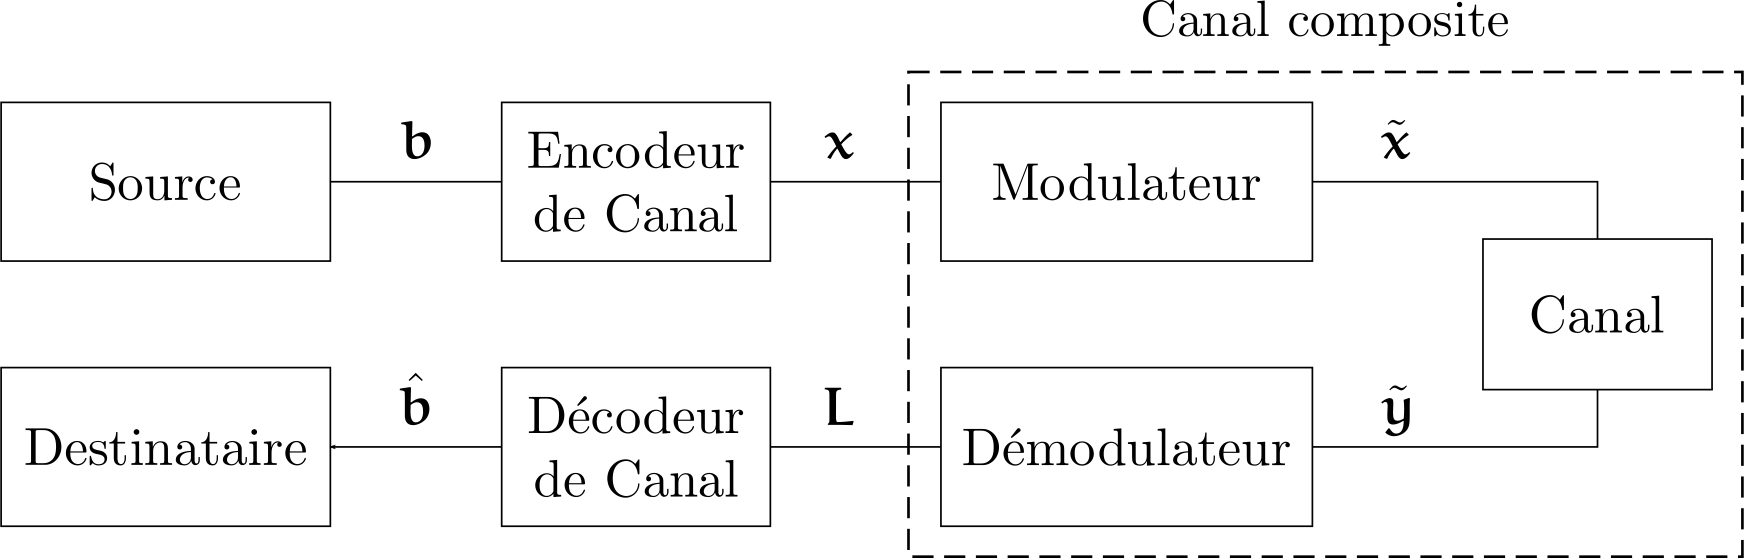
\includegraphics[width=0.8\textwidth]{main/ch1_fig/chaine_com}
\caption{Une chaîne de communication}
\label{fig:chaine_com}
\end{figure}
Une chaîne de communications numériques est représentée en Figure~\ref{fig:chaine_com}.
Elle représente les étapes usuelles de la transmission de données numériques depuis une \textbf{Source} vers un \textbf{Destinataire} à travers un \textbf{Canal}.
Le canal de transmission est le support qui permet le transfert de l'information. Lors de communications sans fil, il s'agit du vide, par lequel passent les ondes émises par les antennes de nos équipements. Or les grandeurs physiques associées à ce canal sont continues tandis que les données à transmettre sont une \textbf{séquence d'information} constituée de bits, donc discrètes. C'est le rôle du modulateur que de transformer ce flux binaire en signaux physiques transmissibles par le canal. Si l'on considère toujours le cas d'application des communications sans fils, le modulateur transforme des séquences de bits en formes d'ondes.

Au sein du canal de communication, les signaux subissent de nombreuses perturbations. Le bruit thermique des composants circuits électroniques de la chaine de transmission et les interférences causées par d'autres utilisateurs du canal sont des exemples de sources de perturbations. Le démodulateur, qui a le rôle inverse du modulateur, c'est-à-dire de convertir les signaux physiques en données binaires, peut, à cause de ces perturbations, commettre des erreurs. Ceci est un problème, puisque le but de la chaîne de transmission est de transmettre au destinataire l'exacte réplique de la séquence d'information donnée par la source. Dans le cas contraire, il s'agit d'erreurs de transmissions. La qualité de la chaine de transmission est souvent mesurée par son taux d'erreur binaire (BER), qui correspond au nombre de bits erronés sur le nombre total de bits transmis.

L'ajout d'un encodeur et d'un décodeur canal dans la chaîne de transmission est un moyen efficace de réduire ce taux d'erreur. L'encodeur transforme une séquence d'information $\mathbold{b}$ de $K$ bits en un \textbf{mot de code} $\mathbold{x}$ de $N$ bits. La taille du mot de code, en nombre de bits, est supérieure à la taille de la séquence d'informations afin d'ajouter de la redondance au message transmis: le rendement du code $R=K/N$ est inférieur à $1$. Cette redondance est utilisée par le décodeur canal, ou parfois le couple démodulateur - décodeur canal, afin de réduire le taux d'erreur binaire de la chaîne de transmission. Dans la présente thèse, le décodeur canal est découplé du démodulateur. L'ensemble modulateur - canal - démodulateur peut être considéré comme une entité indépendante dont l'entrée est le mot de code $\mathbold{x}$ et la sortie une séquence d'estimation $\mathbold{L}$. Cet ensemble est appelé canal composite.

\subsection{Le canal composite}
Un seul et unique modèle de canal composite sera considéré tout au long de ce manuscrit. Sa modulation est une modulation à changement de phase binaire (BPSK) qui associe aux valeurs binaires d'entrée $x\in\{0,1\}$ les valeurs réelles $\hat{x}\in\{-1,1\}$, respectivement.
Le canal à bruit blanc additif gaussien à double entrée (BI-AWGNC) tel que défini dans \cite[Section~1.5.1.3]{ryan2009channel} est considéré. Ce modèle est le plus utilisé pour caractériser les performances des codes correcteurs d'erreur car il se rapproche du bruit thermique évoqué précédemment, qui est souvent prépondérant. Il consiste en l'addition d'une variable réelle à distribution gaussienne centrée en $0$ et de densité spectrale $N_0$. Afin d'évaluer les performances de correction des codes correcteurs d'erreurs, les taux d'erreur seront souvent rapportés à cette densité spectrale, ou plus précisément au \textbf{rapport signal à bruit} (SNR), noté $E_b/N_0$, où $E_b=\frac{\mathbb{E}(\hat{x}^2)}{R}$ est l'énergie moyenne par bit d'information.

Les estimations en sortie du démodulateur sont données sous la forme de rapport de vraisemblance logarithmique (LLR). Leur signe détermine la valeur binaire d'entrée $x$ la plus probable, et leur valeur absolue le degré de fiabilité de cette valeur d'entrée. Des détails sur le modèle de canal et le calcul de ces LLRs sont données en Annexe \ref{append:canal}.

\subsection{Encodage de codes polaires}
Les codes polaires appartiennent à la famille des codes en blocs linéaire. Soient les ensembles $\mathbb{B}^n = \{0,1\}^n$, et  une matrice de taille $G \in \mathbb{B}^K \times \mathbb{B}^N$. L'encodage d'un code en blocs linéaire est une application linéaire injective de $\mathbb{B}^K$ vers $\mathbb{B}^N$ qui à un élément $\mathbold{b} \in \mathbb{B}^K$ associe un élément $\mathbold{x} \in \mathbb{B}^N$ tel que $x=bG$. Définir un encodeur de code polaire revient donc à définir sa matrice génératrice $G$. 

La matrice génératrice d'un code polaire est elle-même produit de deux matrices $E \in (\mathbb{B}^K \times \mathbb{B}^N)$ et $F^{\otimes n}\in (\mathbb{B}^N)^2$, $G=EF^{\otimes n}$. La multiplication par la matrice $E$ correspond à l'ajout de "bits gelés", dont la valeur est $0$, à la séquence d'information $\mb{b}$. Le résultat de l'opération $\mathbold{u} = E\mathbold{b}$ est constitué de $K$ bits $b_i \in \mathbold{b}$ et de $N-K$ bits gelés. Les positions respectives des bits d'informations et des bits gelés sont liés au phénomène de polarisation décrit dans la section suivante est sont déterminants quant à la performance de correction du code.

La matrice $F^{\otimes n}$, où $N=2^n$, est la n-ième puissance de Kronecker du noyau $F=\left[\begin{smallmatrix} 1 & 0 \\ 1 & 1\end{smallmatrix}\right]$. En Figure \ref{fig:encodage} sont données plusieurs représentations de cette matrice d'encodage. La représentation sous forme de \textit{factor graph} est une représentation alternative où les symboles $\oplus$ correspondent à des opération \textit{OU-exclusif}. La représentation sous forme d'arbre binaire est quant à elle particulièrement pertinente pour la description des algorithmes de décodage.

\begin{figure}[t]
\centering
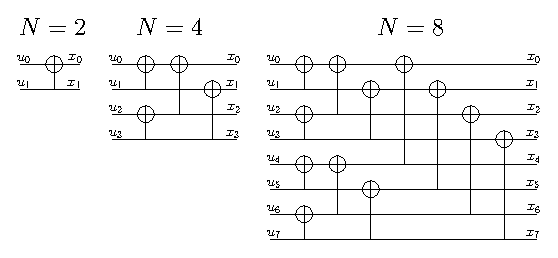
\includegraphics[width=0.7\textwidth]{main/ch1_fig/Graph_N_rec}
\caption{Différentes représentation de l'encodage de codes polaires}
\label{fig:encodage}
\end{figure}

Le processus d'encodage peut également être modifié pour rendre le code systématique. Un code correcteur d'erreur est dit systématique si les bits de la séquence d'information sont présents dans le mot de code. Pour se faire, il faut modifier la matrice d'encodage : $G_{sys}=EF^{\otimes n}EF^{\otimes n}$. Il est alors prouvé dans \cite{arikan_systematic_2011} que si $\mb{x}=\mb{b}G_{sys}$, alors $\mb{b}=E^{-1}\mb{x}$. L'encodage systématique est représenté en Figure \ref{fig:sys}.

\begin{figure}[t]
\centering
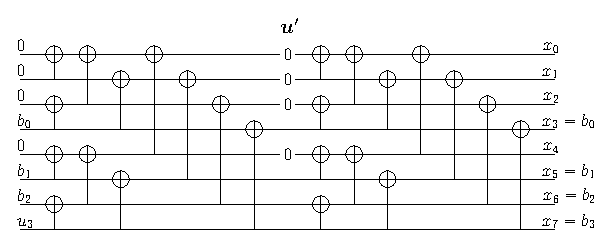
\includegraphics[width=0.7\textwidth]{main/ch1_fig/Graph_N_sys}
\caption{Encodage systématique}
\label{fig:sys}
\end{figure}

\subsection{Polarisation}

L'invention des codes polaires et la définition des matrices d'encodage par Ar{\i}kan \cite{arikan_channel_2009} est lié au phénomène de polarisation. L'ensemble constitué de l'encodeur polaire, du canal composite et du décodeur polaire peut être vu comme un ensemble de canaux de transmission qui chacun transmet un bit. On parle de polarisation parce que, dans ces condition, il est possible de montrer que ces $N$ canaux ont tendance à se diviser en deux groupes. Un groupe de canaux très fiables, avec une probabilité d'erreur faible, et un groupe de canaux peu fiables, à probabilité d'erreur forte. Cette tendance augmente quand $N$ augmente, les canaux se polarisent. Ainsi, les bits d'informations seront attribués aux canaux fiables, et des bits dits gelés, dont la valeur est connue à priori, seront attribués aux canaux peu fiables. Le processus de détermination de la position des bits gelés dans le vecteur $\mathbold{u}$ est appelé construction des codes polaires. Celle-ci est déterminante pour la performance de correction des codes polaires. Plusieurs méthodes efficaces ont été proposées \cite{tal_how_2013,trifonov_efficient_2012} pour le canal AWGN.

\section{Les algorithmes de décodage de codes polaires}

Deux algorithmes de décodages ont été proposés dès l'invention des codes polaires \cite{arikan_channel_2009}. L'algorithme de décodage appelé Annulation Successive (SC) est un algorithme de décodage à sortie dure : les données de sortie sont des bits. L'algorithme de décodage par propagation de croyance (BP) est au contraire un algorithme de décodage à sortie souple, dont les données de sortie sont des estimations représentée par exemple par des LLRs. De nombreuses variantes de ces algorithme ont ensuite été proposées pour améliorer leur performances de corrections. Les algorithme Annulation Successive par Liste (SCL), Annulation Successive "Flip" (SCF), Annulation Sucessive par Pile (SCS) sont des évolutions de l'algorithme SC. Tandis que l'algorithme appelé Annulation Souple (SCAN) eut être vu comme une combinaison des algorithmes SC et BP. Chacun de ces algorithmes est décrit dans cette section.

\subsection{Le décodage par Annulation Successive}

\subsubsection{L'arbre de décodage}
\begin{figure}[t]
\centering
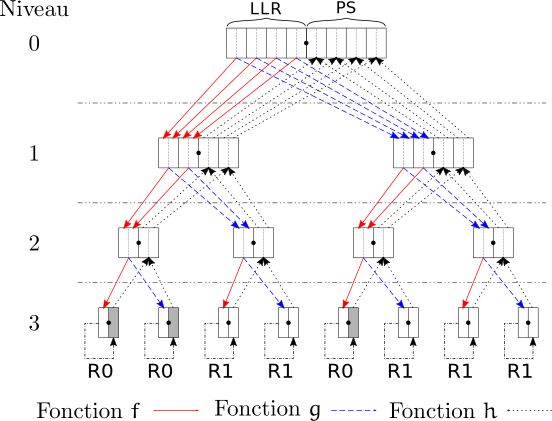
\includegraphics[width=0.7\textwidth]{main/ch1_fig/sc}
\caption{Arbre de décodage SC}
\label{fig:sc}
\end{figure}
% mettre en évidence qu'on décode bit par bit, sera utile pour sc list
% introduire termes rendement 1 / rendement 0
% sommes partielles termes non introduit
% vérifier que n est introduit
Les données d'entrée des algorithmes de décodages présentés ici sont des LLRs, contenus dans le vecteur $\mathbold{L}$ de taille $N$, sortis du canal composite. Les données de sorties sont des bits contenus dans le vecteur $\mathbold{\hat{b}}$ de taille $K$. Au cours du décodage de codes polaires, ces deux formats de données (LLRs et bits) sont également utilisés. La Figure~\ref{fig:sc} représente ces données nécessaires. Dans l'exemple considéré, $K=3$ et $N=8$. Les données sont organisées en arbre binaire sur $log_2(N) + 1$ couches. Dans notre cas donc, l'arbre possède quatre niveaux. A chaque couche sont attribués un certain nombre de noeuds. La racine de l'arbre numérotée $0$ est constituée d'un seul noeud. Ce noeud contient $N$ LLRs et $N$ sommes partielles. En decendant dans l'arbre, à chaque couche, le nombre de noeuds double, tandis que le nombre de LLRs et de sommes partielles de chaque noeud et divisé par deux. Chaque couche $d$ contient $2^d$ noeuds constitués de $2^{n-d}$ LLRs et de $2^{n-d}$ sommes partielles. 

% Ajouter channel LLRs à la racine
\subsubsection{Les fonctions élémentaires et leur séquencement}
La première étape du décodage est le chargement des LLRs du canal $L$ : les LLRs du noeud racine prennent la valeur des LLRs du canal. Les LLRs et les sommes partielles de chaque noeud de l'arbre sont ensuite calculées par l'intermédiaire des opérations $f$, $g$, $h$, \texttt{R0} et \texttt{R1} symbolisées dans la Figure~\ref{fig:sc} par des flèches. Elles correspondent aux équations \ref{eq:sc}. 
\begin{eqnarray}
  \begin{array}{l c l}
    f(L_a,L_b) &=& \text{sign}(L_a.L_b).\min(|L_a|,|L_b|)\\
    g(L_a,L_b,\hat{s}_a)&=&(1-2\hat{s}_a)L_a+L_b\\
    h(\hat{s}_a,\hat{s}_b)&=& (\hat{s}_{a} \oplus \hat{s}_{b}, \hat{s}_{b})\\
    \texttt{R0}(L_a) &=& 0 \\
    \texttt{R1}(L_a) &=&  \left\{\begin{array}{l c l} 0 \text{ si } L_a \geq 0 \\ 1 \text{ si } L_a < 0 \end{array}\right.
  \end{array}
  \label{eq:sc}
\end{eqnarray}
\begin{figure}[b]
\centering
\includegraphics[width=0.5\textwidth]{main/ch1_fig/seq_sc}
\caption{Séquencement du décodage SC d'un code polaire de taille $N=8$.}
\label{fig:seq_sc}
\end{figure}
% Expliciter notation (N,K)
Les fonctions $f$ et $g$ prennent comme entrée des LLRs et produisent des LLRs en sortie. Elles permettent de descendre dans l'arbre jusqu'aux feuilles. Les feuilles sont les noeuds les plus bas de l'arbre. Le traitement d'une feuille correspond à l'application des opérations \texttt{R0} et \texttt{R1}. Lors d'un décodage non systématique, les sommes partielles contenues par les feuilles correspondent aux bits du mot de code. Certains sont donc des bits d'informations, d'autres sont des bits gelés dont la valeur, $0$, est connue d'avance. Pour les feuilles contenant les bits gelés, l'opération \texttt{R0} est appliquée, la somme partielle est égale à 0. Lorsque la feuille contient un bit d'information, l'opération \texttt{R1} est appliquée, la somme partielle est obtenue par seuillage du LLR. Après le décodage d'une feuille, la fonction $h$ est appliquée afin de remonter dans l'arbre. La hauteur jusqu'à laquelle les sommes partielles sont calculées grâce à la fonction $h$ dépend de l'index de la feuille qui vient d'être décodé. Cette recombinaison des sommes partielles est nécessaire à l'application des fonctions $g$, qui prennent en argument des sommes partielles. Le séquencement du décodage SC d'un codes polaire de taille $N=4$ est détaillé en Figure~\ref{fig:seq_sc}. Dans le cas d'un code non systématique, le mot de code décodé se trouve dans les feuilles de l'arbre de décodage. Les opération 12 et 13 dans la Figure \ref{fig:seq_sc} sont donc inutiles puisqu'elles servent seulement à calculer les sommes partielles du noeud racine. Par contre, dans le cas d'un code systématique, ce sont les sommes partielles du noeud racine qui correspondent au mot de code décodé.

\subsubsection{Le parallélisme de l'algorithme}
Dans la Figure~\ref{fig:sc}, quatre fonctions $f$ sont appliquées sur le noeud racine pour calculer les LLRs de la branche de gauche. Ces quatre fonctions sont indépendantes : leurs entrées et sorties sont disjointes. Par conséquence, elles peuvent être réalisées simultanément. Cela est également vrai pour chaque fonction $f$, $g$ et $h$ d'un noeud donné. Ainsi, le niveau de parallélisme est différent selon la couche considérée et correspond à la taille du noeud de sortie. Le parallélisme est donc plus grand en haut de l'arbre qu'en bas. Lorsque ce parallélisme est utilisé, on parle de parallélisme \textit{intra-trame}.


\subsection{Le décodage par Annulation Successive Liste}
\subsubsection{L'algorithme}
L'algorithme de décodage par Annulation Successive Liste (SCL) est une évolution de l'algorithme SC \cite{tal_how_2013}. L'algorithme SC présente en effet des performances de correction médiocres pour des codes polaires de petite taille. Le SCL améliore ses performances substantiellement. Dans l'algorithme de décodage SC décrit précédemment, des décisions dure sont réalisées à chaque décodage d'une feuille correspondant à un bit d'information (fonction \texttt{R1}). Si une erreur est commise au sur une feuille lors de ce seuillage, celle-ci est irréversible, et le décodage du mot de code est un échec. Le principe de l'algorithme de décodage par liste est de retarder la décision dure. Au lieu d'appliquer un seuillage sur la valeur du LLR, les deux possibilités de décodage sont considérées, et l'arbre de décodage, avec l'ensemble de ses LLRs et sommes partielles, est dupliqué. Le décodage continue ainsi sur les deux arbres parallèlement. A chaque feuille de rendement 1, le même procédé est réalisé, doublant le nombre d'arbres décodés en parallèle.

% citer article balatsoukas
% Ajouter les bits décodés sur les arbres pour les faire apparaître lors de la description du liste. 
Il n'est pas possible, en pratique, de dupliquer indéfiniment le nombre d'arbres de décodage, la mémoire nécessaire et le nombre de calcul devient vite insoutenable. Un nombre de chemins maximum $L$ paramétrise donc l'algorithme liste. La sélection des chemins qui seront conservés ou éliminés est réalisée grâce à une métrique $m$ associée à chaque chemin. Cette métrique est mise à jour à chaque traitement d'une feuille. Lorsque la feuille est de rendement 0 si le LLR de la feuille est positif, la métrique est inchangée car l'estimation du LLR est en encore avec la valeur du bit gelé, 0. Si le LLR est négatif alors au contraire, la valeur absolue du LLR lui est ajoutée. Lorsque la feuille est de rendement un, deux chemins sont créés, avec chacun une version différente du bit décodé. Le chemin créé dont la valeur du bit est en accord avec la valeur du LLR ne reçoit pas de pénalité. Au contraire, la métrique du deuxième chemin créé est accrue de la valeur du LLR.

Une fois ces calculs de métriques réalisés, on sélectionne les chemins à conserver. Si $L$ chemins étaient actifs au moment du traitement d'une feuille de rendement 1, alors $2L$ chemins sont générés, avec chacun une métrique associée. Seuls les $L$ chemins avec la métrique la plus faible sont conservés. A la fin du parcours de l'arbre de décodage, $L$ chemins auront donc été conservés. Ces $L$ chemins correspondent à $L$ mots de codes possibles. Une sélection d'un seul candidat parmis les $L$ doit être effectuée. Dans la version originale de l'algorithme, le mot décodé associé au chemin ayant la métrique de valeur la plus faible à la fin du décodage est sélectionné comme étant la sortie de l'algorithme $\mathbold{\hat{b}}$.

\subsubsection{Concaténation avec un CRC}
Les auteurs de \cite{tal_how_2013} ont proposé de concaténer un test de redondance cyclique (CRC) pour discriminer les différents candidats. A la fin de l'algorithme de décodage, lorsque les $L$ mots de codes sont disponibles, un CRC est appliqué sur chacun d'entre eux. Si l'un d'entre eux vérifie le CRC, il est alors hautement probable qu'il soit le bon candidat. Le mécanisme est illustré en Figure~\ref{fig:crc}.

% Prendre une décision sur l'appellation des algos (de / par / [] Annu Succ par / "" / [] Liste / Pile)
% Pour chaque algo, lister possiblement les améliorations mineures

\subsection{Autres algorithmes}
	L'algorithme de décodage par Annulation Successive Flip (SCF) \cite{afisiadis_low-complexity_2014} est une variante de l'algorithme SC. Il vise également à améliorer les performances de décodage. Cet algorithme nécessite la concaténation d'un CRC pour être réalisé. L'algorithme de décodage SC est appliqué une première fois. L'ensemble des LLRs permettant les décisions dure (les LLRs des feuilles) est conservé. Si le mot de code décodé satisfait le CRC, alors le décodage s'arrête. Par contre, si le CRC n'est pas satisfait, alors l'algorithme SC est lancé une nouvelle fois. La différence est que la décision prise, lors du premier décodage, sur le LLR le moins fiable est inversée. Ce deuxième mot décodé est encore testé à l'aide du CRC. S'il ne satisfait toujours pas le CRC, une autre séquence de décodage est lancée en inversant le bit du deuxième LLR le moins fiable. Ce mécanisme itératif continue jusqu'à un nombre d'essai maximum $T$.


	% SC Stack
	L'algorithme de décodage par Annulation Successive Pile (SCS) \cite{chen_improved_2013} est une variante de l'algorithme SCL. Dans l'algorithme SCL, le nombre de candidat $L$ est conservé stable tout au long de l'algorithme. De plus, le séquencement est exactement le même que dans le SC dans les différents arbres décodés parallèlement : les feuilles sont décodées l'une après l'autre, dans l'ordre. Dans l'algorithme SCS, les métriques associées aux différents arbres de décodages sont maintenues dans une pile ordonnée de profondeur $T$. L'algorithme SC est appliqué sur le chemin associé à la meilleure métrique. A l'arrivée sur une feuille, la métrique de l'arbre est mise à jour et, si la feuille est de rendement 1, un nouveau chemin est ajouté à la pile. \`A un instant $t$, seul l'arbre étant le plus haut sur la pile est décodé. Lorsque la dernière feuille de l'un des chemins est décodé, le CRC est testé. Le décodage se termine lorsqu'un mot décodé satisfait le CRC ou que le nombre de candidats testés atteint une valeur déterminée à l'avance $D$. L'algorithme SCS présente l'avantage de nécessiter moins d'opérations élementaires sur les codes polaires. Cependant, le maintien d'une pile et son séquencement particulier rendent son implémentation difficile.
	% Citer Harsch
	% Parler du Stack Hybride ? 


\subsection{Algorithmes itératifs à sortie souple}

\subsubsection{L'algorithme de décodage à Propagation de Croyance}
Les algorithmes cités précédemment sont des algorithmes de décodage à sortie dures. Leur sortie consiste en un mot de code décodé $\mathbold{\hat{b}}$ constitué de bits. Certains algorithmes permettent au contraire de générer des sorties souples représentant des vraisemblances. Dans nos exemples celles-si prendront la forme de LLRs. Lors de l'invention des codes polaires \cite{arikan_channel_2009}, le premier algorithme à sorties souples proposé fut l'algorithme de décodage à Propagation de Croyance (BP). Au contraire de l'algorithme SC, aucune décision dure n'est effectuée au cours du décodage. Les sommes partielles sont remplacées par des LLRs. Les fonction utilisées pour les calculs des LLRs sont listées dans les Equations \ref{eq:bp}.
    \begin{eqnarray}
      \begin{array}{l c l}
        f_{bp}(L_a,L_b,L_c) &=& f(L_a, L_b + L_c) \\
        g_{bp}(L_a,L_b,L_c)&=& f(L_a, L_c) + L_b
      \end{array}
      \label{eq:bp}
    \end{eqnarray}

\begin{itemize}
\item Noeud 2 à sortie souple
\item BP
\item SCAN
\end{itemize}


\subsection{Comparaisons des algorithmes}
\begin{itemize}
	\item SCS
	\item SCF
\end{itemize}

\section{Améliorations algorithmiques}

\subsection{Elagage de l'arbre de décodage}

\subsubsection{Fast SC}
\begin{itemize}
\item R0 - R1
\item SPC - REP
\item détailler calculs évitables (g0, f0, grep)
\end{itemize}
\subsubsection{Fast SCL}
\begin{itemize}
\item détailler adaptation élagage pour SC Liste - calculs métriques
\item discussion chase spc - r1 ? Hashemi-Sarkis + Simulations
\end{itemize}
\subsubsection{Fast SCAN}
\begin{itemize}
\item 
\end{itemize}

\subsection{Adaptive}

\section{Codes polaires de taille variables}
% https://arxiv.org/pdf/1701.06458.pdf 4-5-6-7-8-9


\subsection*{Conclusion}
             % Premier thème (Doctorat) ou "Détails de la Solution" (Maîtrise).
%!TEX root = ../my_thesis.tex
\chapter{Décodeurs logiciels des algorithmes "Liste"} % (fold)

% Intro chapitre

\vspace*{\fill}
\minitocTITI
\vspace*{\fill}
\newpage


\section*{Introduction}

\section{Etat de l'art des implémentations logicielles d'algorithmes de codes polaires}

\subsection{Vectorisation}
\subsection{Déroulage}
\subsection{Cibles}

\section{Généricité et Flexibilité d'un décodeur de codes polaire}

\subsection{Définitions}
\subsection{Réalisation}
\subsection{Exploration}

\section{Optimizations de l'implémentation logicielle des décodeurs liste}

\subsection{Algorithmes de tri}
\subsection{Accélération du contrôle de redondance cyclique}
\subsection{Gestion des sommes partielles}

\section{Expérimentations et mesures}

\subsection{Comparaison des cibles}
\subsection{Comparaison des algorithmes}
\subsection{Comparaison avec l'état de l'art}
 
\section*{Conclusion}
             % Second thème (Doctorat) ou "Résultats théoriques et expérimentaux" (Maîtrise).
%!TEX root = ../my_thesis.tex
\chapter{Conception d'un processeur par la spécialisation d'une architecture de base.} % (fold)
\label{chap:tensilica}

\vspace*{\fill}
\minitocTITI
\vspace*{\fill}
\newpage

\section*{Introduction}
Afin de tendre vers un réseau virtualisé de type Cloud-RAN, les implémentations logicielles des fonctions de traitement du signal dans les infrastructures de communication radio sont encouragées. Dans le chapitre précédent, de telles implémentations sont présentées pour les algorithmes de décodage polaire à liste. De hauts débits peuvent être atteints, et la flexibilité et la généricité de ces décodeurs sont très importantes. En utilisant des processeurs visant des systèmes électroniques embarqués, ces implémentations peuvent également gagner en efficacité énergétique.

Toutefois, les processeurs à usage général incluent de nombreuses unités matérielles destinées à exécuter efficacement de nombreuses et diverses applications. Mais toutes les unités matérielles ne sont pas utilisées dans la plupart des applications. Par exemple, dans les algorithmes de décodage de canal, toutes les unités de calcul à virgule flottante sont inutiles puisqu'une représentation des données internes en virgule fixe est privilégiée. Ces unités matérielles consomment alors de l'énergie inutilement. Le profilage d'un décodeur polaire montre que la majeure partie du temps d'exécution est passé à réaliser un ensemble restreint de fonctions élémentaires. De plus, une part significative des instructions exécutées correspond à des opérations de sauvegarde et de chargement de données dans les registres.

Ces observations poussent à envisager la conception d'un processeur programmable qui exclurait les unités matérielles inutiles des processeurs à usage général, tout en intégrant des unités de calculs spécialisées dans la réalisation efficace des fonctions élémentaires de décodage de codes polaires. Une telle architecture doit permettre de conserver une grande flexibilité nécessaire à la virtualisation des réseaux, tout en garantissant un niveau de performance se rapprochant des architectures dédiées. Ce type de processeurs entre dans la catégorie des processeurs à jeu d'instructions spécifique à l'application (ASIP: Application Specific Instruction-set Processor).

Les Chapitres \ref{chap:tensilica} et \ref{chap:tta} de ce manuscrit présentent deux architectures de processeurs ASIP spécialisées dans le décodage de code polaire. Ces deux architectures ont été conçues selon des méthodologies de conception différentes. La première méthodologie développée dans ce chapitre correspond à la spécialisation d'un processeur de base. Dans la section \ref{sec:asips}, le concept d'ASIP est introduit, et la méthodologie utilisée pour la première architecture est décrite. Dans la section \ref{sec:tensilica_design}, la conception de l'ASIP est détaillée. Enfin les résultats d'implémentation et les performances de l'architecture en termes de débit, latence, complexité matérielle et consommation énergétiques sont présentés et discutés dans la section \ref{sec:tensilica_res}.


\section{Les processeurs à jeu d'instructions spécifique à l'application}
\label{sec:asips}

Une des architectures ASIP que nous avons développées est basée sur un processeur de type RISC (Reduced Instruction Set Computer). Dans une première sous-section, les principes des architectures RISC sont présentés. Le concept d'ASIP est ensuite introduit. Les méthodologies de conceptions d'ASIP peuvent être divisée en deux groupes que nous détaillons. Le flot de conception de l'outil logiciel retenu pour concevoir ce premier ASIP sera ensuite présenté.

\subsection{Les processeurs RISC}
\label{subsec:risc}
\begin{figure}[t]
\centering
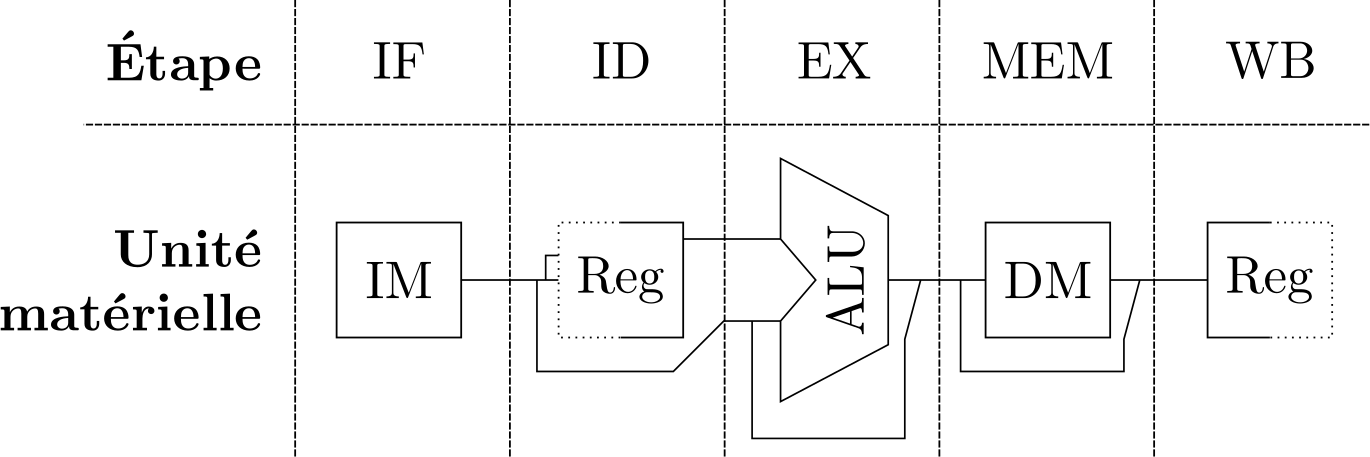
\includegraphics[width=\textwidth]{main/ch3_fig/stages}
\caption{\'Etages d'un processeur RISC}
\label{fig:risc}
\end{figure}

Dans le domaine de l'embarqué, les processeurs utilisés sont souvent de type RISC. Cette classe de processeurs a été introduite dans \cite{hennessy2011computer}. Par une analyse statistique et quantitative des applications traitées par les architectures de processeurs, les auteurs ont abouti à une microarchitecture de processeurs composée de 5 étages. Une unité matérielle est associée à chacun des étages, comme montré dans la Figure \ref{fig:risc}.

\begin{itemize}
  \item Le premier étage est l'étage de \textbf{chargement de l'instruction} (IF : Instruction Fetch) depuis la \textit{mémoire d'instruction} (IM : Instruction Memory). A chaque cycle d'horloge, une nouvelle instruction est chargée dans un registre spécialisé, nommé registre d'instruction. L'adresse en mémoire de l'instruction à charger est déterminée par le pointeur d'instruction, registre incrémenté automatiquement à chaque cycle d'horloge. L'instruction détermine l'opération qui à effectuer par le processeur dans les étages suivants. Il peut s'agir d'instructions arithmétiques et logiques, d'instructions de chargement et de sauvegarde depuis et vers la mémoire, ou bien d'instructions de branchement et de sauts. Ces dernières permettent de se déplacer dans la mémoire d'instructions. L'instruction contient également des informations sur les registres qui doivent être lus ou écrits, ainsi que des adresses mémoire dans le cas d'opérations de chargement ou de sauvegarde.

  \item Le deuxième étage correspond au \textbf{décodage de l'instruction} (ID : Instruction Decode) et à la lecture de la \textit{file de registres} (RF : Register File) spécifié(s) par l'instruction. Divers signaux de contrôle, qui seront utilisés dans les étages suivants, sont générés, selon l'instruction décodée.

  \item Le troisième étage est l'étage d'\textbf{exécution} (EX : Execution) dans lequel l'unité arithmétique et logique (ALU : Arithmetical and Logical Unit) effectue des opérations arithmétiques (+,-,*,/) et logiques (AND, OR, XOR,...). Ces opérations peuvent servir a effectuer des calculs d'adresses relatives ou à réaliser des opérations sur deux opérandes. Ces deux opérandes peuvent être deux registres ou bien un registre et une valeur immédiate intégrée dans l'instruction elle-même.

  \item Le quatrième étage est l'étage d'\textbf{accès à la mémoire}. S'il s'agit d'un chargement, une donnée est lue dans la \textit{mémoire de donnée} (DM : Data Memory) à l'adresse spécifiée dans un des registres. S'il s'agit d'une sauvegarde, la valeur d'un deuxième registre est écrite dans la DM.

  \item Le cinquième étage est l'étage d'\textbf{écriture différée} (WB : write-back). Cette étage permet d'écrire le résultat dans la file de registres, que ce soit le résultat d'une opération effectuée par l'ALU ou bien une donnée lue dans la DM.
\end{itemize}

\begin{figure}[t]
\centering
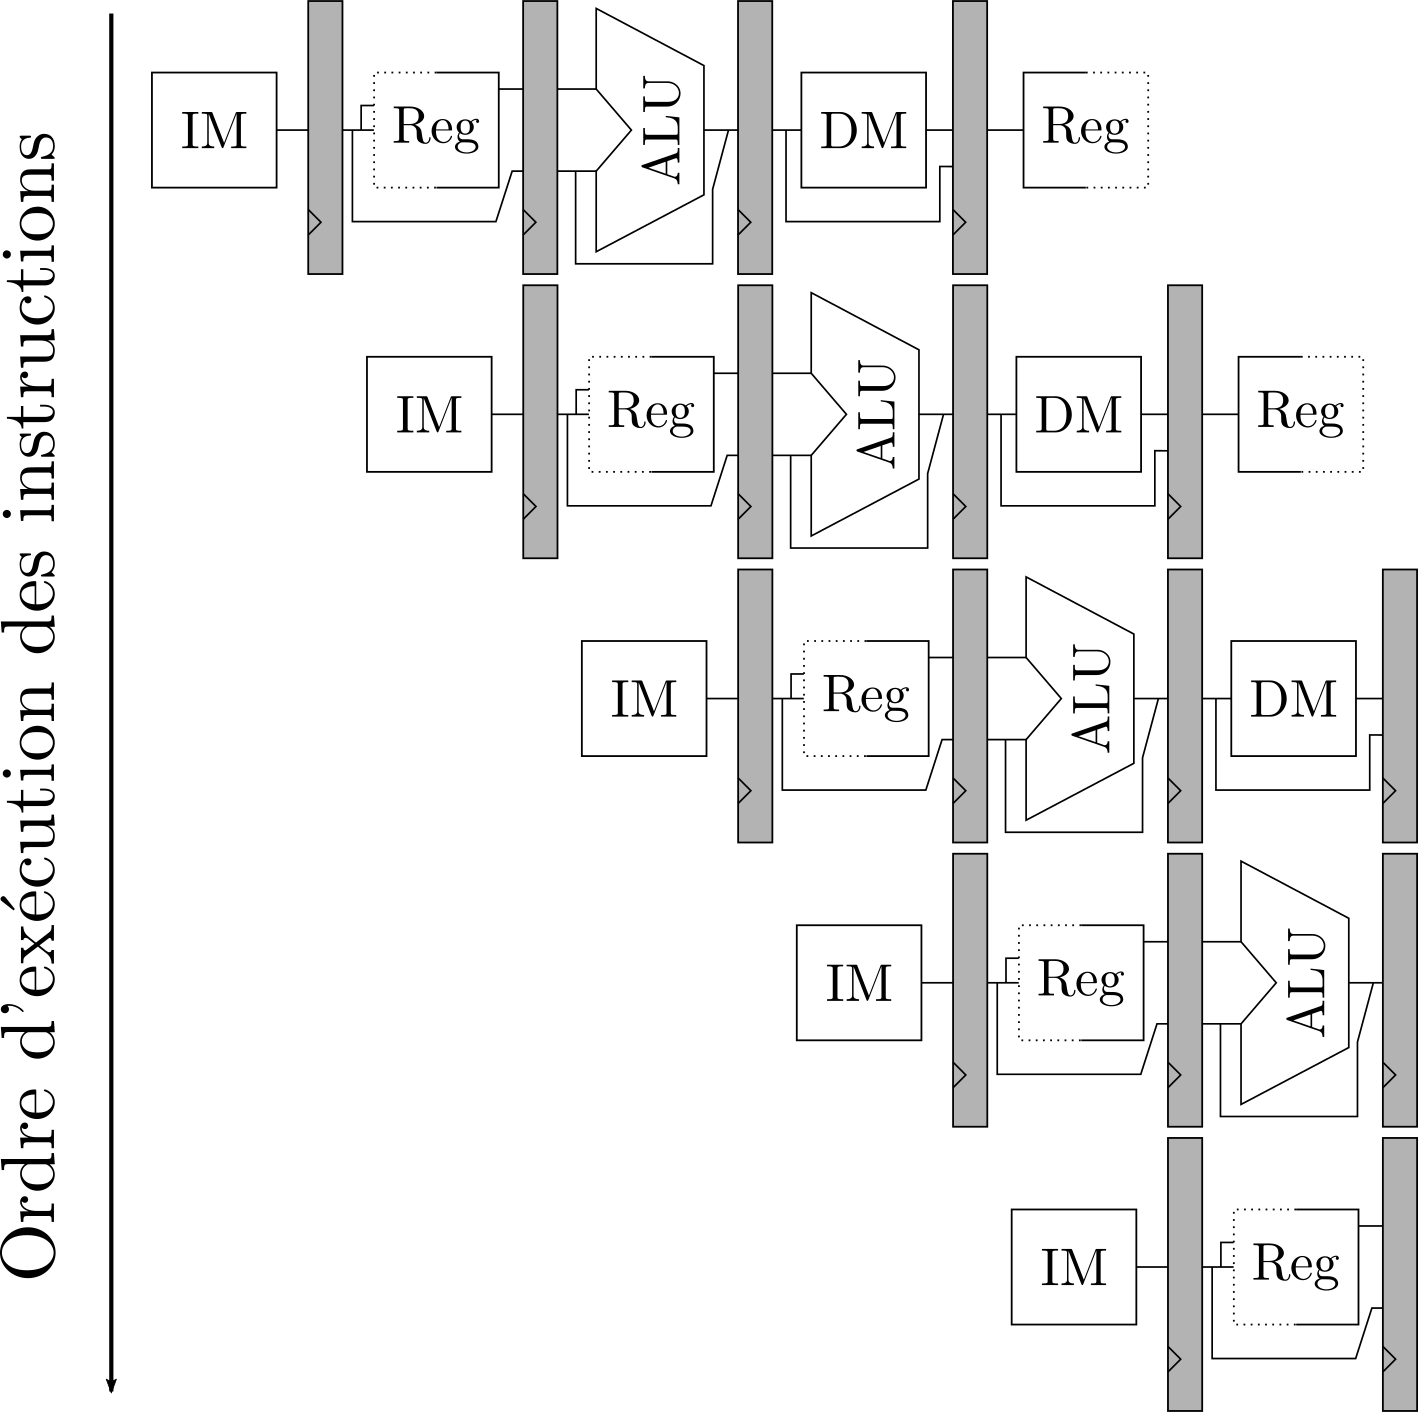
\includegraphics[width=0.75\textwidth]{main/ch3_fig/pipelines}
\caption{Structure et fonctionnement du pipeline RISC classique à 5 étages.}
\label{fig:pipelines}
\end{figure}


L'ajout de registres de pipeline comme illustré dans la Figure~\ref{fig:pipelines} permet d'isoler chacun des étages. Ainsi à chaque cycle d'horloge, une instruction est transmise d'un étage au suivant. Si une instruction est initiée à chaque cycle d'horloge, alors la performance du processeur sera 5 fois supérieure à celle d'un processeur sans registre de pipeline.

Nous venons d'introduire l'architecture RISC telle que définie dans \cite{hennessy2011computer}. Cette dernière fait figure de référence dans le domaine des architectures de processeur. En effet, cette organisation en pipeline à cinq étages, à quelques différences près, se retrouve actuellement dans de nombreux processeurs. L'architecture de base des processeurs XTensa proposés dans ce chapitre est une architecture de type RISC. Les processeurs XTensa sont une gamme de processeurs proposée par Tensilica, filiale de la société Cadence Design Systems.

\subsection{Les processeurs à jeu d'instructions spécifique à l'application}

Les méthodologies de conception des ASIP peuvent être divisées en deux famille. La première famille correspond à un flot de conception basé sur la spécification complète du processeur, représentée dans la Figure \ref{fig:methodo_adl}. Le modèle du processeur est décrit dans un langage de description architecturale (ADL : Architecture Description Language) \cite{mishra2011processor}. Ces langages de description permettent de définir précisément l'architecture d'un processeur. Ils peuvent être de différents types. Les ADLs structurels décrivent les composants des processeurs ainsi que leurs interconnexions. Les ADLs comportementaux décrivent quand à eux le comportement du jeu d'instructions du processeur. Des langages de description mixtes permettent quant à eux de décrire simultanément la structure et le comportement du processeur. Le flot de conception utilisé pour concevoir le processeur décrit dans le Chapitre \ref{chap:tta} utilise des ADLs comportementaux et structurels afin de générer le modèle matériel du processeur.


\begin{figure}[]
  \centering
  \subfloat[Flot basé sur la spécification complète du processeur.]{
  \includegraphics[scale=0.83]{main/ch3_fig/methodo_a}
  \label{fig:methodo_adl}
  }
  \\
  \subfloat[Flot basé sur la particularisation d’un processeur de base]{
  \includegraphics[scale=0.83]{main/ch3_fig/methodo_b}
  \label{fig:methodo_tensilica}
  }
  \caption{Méthodologies de conception des ASIP}
  \label{fig:asip_methods}
\end{figure}


La deuxième famille de méthodologies représentée dans la Figure \ref{fig:methodo_tensilica} correspond à l'approche utilisée par les outils de Tensilica pour concevoir l'ASIP proposé dans ce chapitre. Une architecture peu complexe en terme de surface occupée et à faible consommation constitue la brique de base du processeur. Dans le cas des outils de Tensilica, cette base est un processeur RISC doté d'un pipeline de 5 étages, tel que présenté dans la sous-section \ref{subsec:risc}. Afin de spécialiser le processeur, deux axes de conception sont disponibles. Premièrement, les principales unités matérielles du processeur RISC désignées dans la Figure \ref{fig:risc} sont paramétrables. Des caractéristiques telles que la profondeur et la largeur de la file de registre et / ou l'interface avec les mémoires sont modifiables. Comme indiqué sur la Figure \ref{fig:methodo_tensilica}, certaines fonctionnalités peuvent être ajoutées ou supprimées : unité de traitement reposant sur des représentations en virgule flottante (FPU : Floating Point Unit), unité d'accélération des multiplications (MUL) ou des divisions (DIV)... Le second axe est la possibilité d'étendre le jeu d'instructions. Grâce à un langage de description matérielle propre aux outils de Tensilica (TIE : Tensilica Instruction Extension) \cite{tie2017reference}, il est possible de spécialiser le processeur pour le décodage de codes polaires en ajoutant des unités matérielles dédiées aux fonctions élémentaires $f$, $g$et $h$.

Un des objectifs de la conception de processeurs par les méthodologies des conceptions que nous venons de présenter est de réduire le temps de conception des systèmes. Pour cela, des étapes clés dans la conception des processeurs sont automatisées. En effet, les suites logicielles de conception d'ASIPs permettent la génération automatique du compilateur, du simulateur, d'un outil de profilage et d'un outil de débogage. 

La génération du compilateur demeure critique. En effet, l'effort à déployer pour créer un compilateur associé à un processeur spécifique est considérable. En revanche, les compilateurs associés aux outils de conception d'ASIPs sont capables de s'adapter aux changements de structure du processeur. Ils proposent des optimisations spécifiques à la structure. Ils doivent également être capable de s'adapter au nombre de registres et les utiliser efficacement. Nous verrons dans le cas de notre processeur spécialisé dans le décodage de codes polaires que l'augmentation du nombre de registres à usage général favorise l'augmentation du débit de décodage. Le compilateur doit également être capable de gérer des modifications du pipeline et permettre un parallélisme d'instructions.

Le simulateur et l'outil de profilage générés permettent la validation fonctionnelle de l'architecture et du programme associé. Le nombre de cycles nécessaires à l'exécution du programme est obtenue à l'aide du simulateur. L'outil de profilage fournit des informations importantes sur la durée de l'exécution de sous-parties du programme afin de cibler les sections les plus consommatrices en temps. Ces métriques déterminent d'éventuelles modifications à apporter pour concevoir un nouveau modèle du processeur. L'outil de conceptions d'ASIP générera alors de nouveau un compilateur, un simulateur et un outil de profilage pour extraire les nouvelles métriques. Des itérations successives de ce flot permettent d'améliorer progressivement les performances recherchées de l'architecture et du programme considérés. Ce processus serait difficilement réalisable sans une telle suite d'outils automatisés.

Une fois l'architecture du processeur déterminée, le modèle matériel du processeur est généré. Ce modèle matériel peut être synthétisé et implémenté sur différentes cibles, ASIC ou FPGA. Il est alors possible d'extraire les métriques d'implémentations : fréquence de fonctionnement, surface occupée, puissance dissipée. De nouveau, des itérations sont possibles afin d'améliorer progressivement les performances.
Pour le processeur XTensa conçu dans le cadre de cette étude, la génération du modèle RTL n'a pas été possible par défaut de licence suffisante de l'outil de conception d'ASIPs. Seules des estimations de fréquence, de surface et de puissance dissipée sont fournies par l'outil. Cette absence de modèle matériel a été une des raisons pour lesquelles nous avons retenu par la suite d'autres méthodologies de conception telles que celle décrite dans le Chapitre \ref{chap:tta}.

\section{Un ASIP dédié au décodage de codes polaires}
\label{sec:tensilica_design}
\subsection{Paramétrage du processeur de base}
\subsubsection{Architecture de base}
La philosophie de conception de l'ASIP proposé est de réaliser l'ensemble des fonctions arithmétiques élémentaires pour le décodage de codes polaires à l'aide d'unités matérielles spécialisées. \`A l'inverse, les opérations de contrôle sont effectuées par l'architecture de référence du processeur XTensa. C'est la raison pour laquelle, l'architecture de référence a été simplifiée. Ainsi, les unités de calcul évoluées (unité de calcul en virgule flottante, MAC, ...) ont été supprimées.

\begin{figure}
\centering
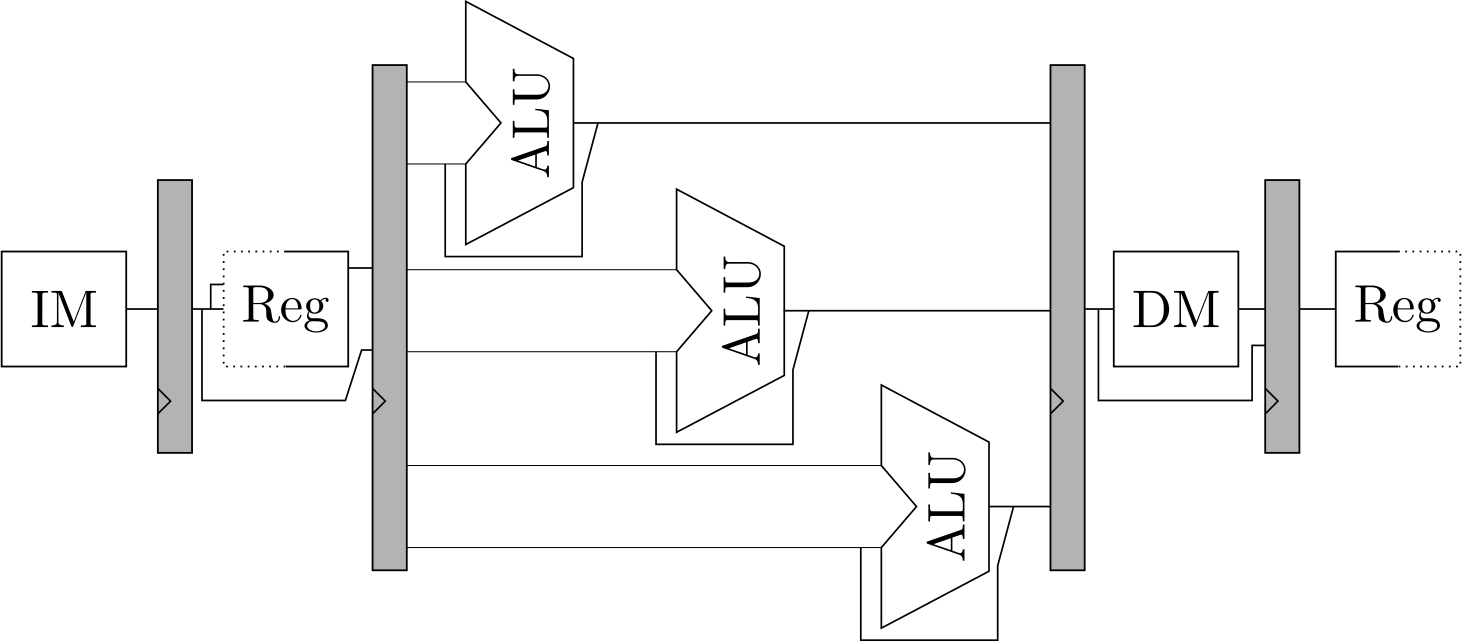
\includegraphics[width=\textwidth]{main/ch3_fig/flix}
\caption{Architecture associée à la fonctionnalité FLIX.}
\label{fig:flix}
\end{figure}

La fonctionnalité FLIX correspond à la possibilité d'ajouter des ALUs supplémentaires à la structure pipeline principale des processeurs XTensa. Cela permet au processeur d'exécuter plusieurs instructions en parallèle. Il est possible de configurer les instructions réalisées par chaque niveau pipeline. Notre choix s'est porté sur une configuration nommée FLIX3 prédéfinie par l'outil de conception. Ainsi, trois instructions faisant partie du jeu d'instruction de base peuvent être appliquées simultanément sur trois couples de données de 32 bits. Ce parallélisme d'instructions permet de réaliser plus rapidement les fonctions de contrôle et de calcul d'adresse. La fonctionnalité FLIX est détaillée dans la Figure \ref{fig:flix}.
La profondeur de la file de registres a été augmentée de 32 à 64 données de 32 bits. Cette modification permet une meilleure exploitation de l'augmentation du parallélisme d'instructions.

\subsubsection{Quantification des données}
Il est démontré dans \cite{sarkis_fast_2014} que des LLRs représentés sur 6 bits permettent d'atteindre les performances de décodage d'implémentations en virgule flottante. Cependant, il est plus simple dans une implémentation logicielle de représenter ces données sur 8 bits puisque les langages de programmation définissent de tels types de données. Comme montré dans \cite{leroux_hardware_2011}, $2^{n-d}$ LLRs doivent être stockés à un niveau $d$ de l'arbre de décodage. La taille de la mémoire permettant de stocker les LLRs est donc de $2^{n+1}-1$ octets.

Les sommes partielles sont des valeurs binaires. Cependant, encore une fois, la manipulation des sommes partielles dans le langage de description logicielle est plus aisée si un entier de 8 bits est utilisé pour représenter chaque somme partielle. Il serait cependant possible d'utiliser un entier pour représenter 8 sommes partielles, ce qui réduirait l'empreinte mémoire de celles-ci. Cependant cela nécessiterait cependant des opérations de masquage supplémentaires et cela introduit plus d'irrégularités au niveau des accès aux données.

\subsubsection{Configuration de la mémoire cache}
\begin{figure}
\centering
\includegraphics[width=\textwidth]{main/ch3_fig/curves/memory/tikz/memory}
\caption{Nombre d'échecs d'accès à la mémoire cache en fonction de la taille de la mémoire pour le décodage SC d'un code polaire de taille $N=1024$.}
\label{fig:tensilica_mem}
\end{figure}

Nous avons fait le choix d'augmenter au maximum le parallélisme des instructions élémentaires nécessaires au décodage de codes polaires. La taille maximum des registres du processeur XTensa, qui est donc la taille utilisée dans l'ASIP proposé, est de 512 bits. Afin de pouvoir charger et sauvegarder des données depuis et vers la mémoire cache en un seul cycle d'horloge, la largeur choisie pour une ligne de mémoire cache est également de 512 bits. La taille de ces mémoires ainsi que leur associativité est également configurable. Des expérimentations ont été réalisées afin de sélectionner les valeurs. Il en résulte qu'une associativité à 4 voies pour les mémoires d'instructions et de données permet d'atteindre de meilleures performances.

Le scenario envisagé pour la conception du processeur est celui des canaux de contrôle du standard 5G tel que défini dans \cite{3gpp_ts_2017}. La taille du plus grand code polaire à décoder est $N=1024$. Les mémoires du processeur ont donc été dimensionnées en conséquence.
Bien que le plus petit nombre d'échec d'accès à la mémoire cache soit atteint pour la taille de cache la plus grande (128 Ko), une mémoire d'instruction de 8 Ko ainsi qu'une mémoire de données de 8 Ko sont suffisantes pour atteindre un nombre d'échecs de cache seulement 10 \% plus grand que la valeur optimale. Les mesures réalisées sont reportées dans la Figure \ref{fig:tensilica_mem}

\subsection{Ressources calculatoires utilisées dans les implémentations matérielles de l'état-de-l'art.}
\label{subsec:hard_sc}

\begin{figure}[t]
\centering
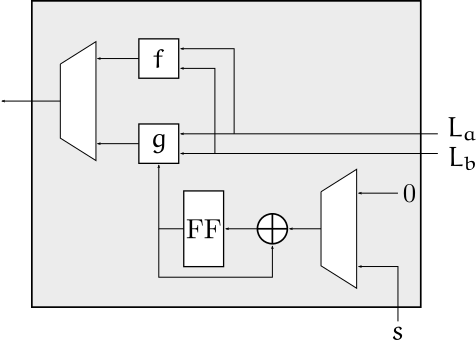
\includegraphics[scale=0.75]{main/ch3_fig/PE}
\caption{Unité matérielle élémentaire (PE : Processing Element).}
\label{fig:pe}
\end{figure}


Les instructions spécialisées choisies pour étendre le jeu d'instructions de l'ASIP s'inspirent des unités de traitement développées dans la littérature pour les circuits dédiés au décodage de codes polaires SC. Dans \cite{leroux_hardware_2011} plusieurs architectures furent proposées. La première architecture est l'architecture dite \og papillon \fg. Lors du décodage, les fonctions $f$ et $g$ doivent être appliquées $N/2$ fois à chaque niveau de l'arbre. Au total, il est nécessaire d'appliquer $\frac{N}{2} \log N$ fois les fonctions $f$ et $g$ lors du décodage d'un mot de code. 

Pour cela, des unités matérielles élémentaires (PE : Processing Elements) ont été définies.
Un PE permet de réaliser un calcul de $f$ ou un calcul de $g$. Un tel élément est représenté dans la Figure \ref{fig:pe}.
Dans l'architecture dite \og papillon \fg, un PE est associé à chaque application des fonctions $f$ et $g$.
Il y a donc au total $\frac{N}{2} \log N$ PEs.
L'application de l'ensemble des fonctions $f$ ou des fonctions $g$ d'un \noeud de l'arbre est alors effectué en un cycle d'exécution.

Cependant, cette architecture est sous-optimale en termes de complexité matérielle.
L'ordonnancement de l'algorithme de décodage SC possède les propriétés suivantes :
\begin{itemize}
  \item Le nombre maximum de fonctions polaires élémentaires pouvant être réalisées simultanément sur un \noeud est $\frac{N}{2}$,
  \item deux \noeuds successifs ne peuvent pas être traités simultanément.
\end{itemize}
En conséquence, les ressources de calcul allouées au traitement d'un \noeud de l'arbre peuvent être utilisées pour le traitements des \noeuds suivants.
Le niveau de parallélisme le plus élevé est $\frac{N}{2}$, donc $\frac{N}{2}$ PEs suffisent pour décoder l'ensemble de l'arbre sans impacter la latence de décodage.
Dans le cas de l'architecture dite \og ligne \fg, $\frac{N}{2}$ PEs sont partagées pour le traitement de tous les \noeuds de l'arbre. Sa latence est la même que celle de l'architecture dite \og papillon \fg.

Dans \cite{leroux_semi-parallel_2013} il est proposé de réduire le nombre de PEs grâce à l'introduction d'une architecture semi-parallèle. Cette architecture s'inspire d'implémentations pour le décodage de codes LDPC \cite{1049697}. Dans un décodeur dit \og ligne \fg, les N / 2 PEs ne sont utilisés simultanément que deux fois durant le décodage d'un mot de code. Cela signifie que le taux d'utilisation des PEs est très faible. Il est donc possible de réduire le nombre de PEs sans impacter significativement le débit.
Cette réduction modifie légèrement l'ordonnancement de l'algorithme de décodage. En effet, les \noeuds nécessitant un nombre d'exécutions de fonctions polaires supérieures à $P$ nécessiteront plus d'un cycle d'horloge à décoder. Le rapport du nombre de PEs d'une architecture semi-parallèle sur le nombre de PEs d'une architecture \og ligne \fg est alors $N/2P$. Par exemple, pour $N=1024$ et $P=64$, le nombre de PEs est réduit d'un facteur $16$, tandis que le débit est seulement réduit de $2\%$. Pour $N=2^{20}$ et $P=64$, le nombre de PEs est réduit d'un facteur $8192$, et le débit est réduit de moins de $10\%$. L'architecture semi-parallèle s'avère donc très pertinente.

L'architecture de décodage proposée dans \cite{sarkis_fast_2014} reprend le principe de l'architecture semi-parallèle. Cependant, les PEs sont modifiés pour intégrer des unités matérielles de traitement des \noeuds spécialisés \texttt{R1}, \texttt{SPC} et \texttt{REP}. Les PEs contiennent également une unité particulière \texttt{REP-SPC} permettant d’accélérer le traitement de deux \noeuds \texttt{REP} et \texttt{SPC} voisins. Ce motif particulier apparaît régulièrement pour le code polaire (32768,29492) considéré dans la publication. Les unités \texttt{REP-SPC} ne sont pas utilisées dans le processeur proposé car elles n'apportent pas de gain significatif pour les tailles de codes traitées dans le cadre du standard 5G, à savoir $N<1024$.

Le dernier type de calcul nécessaire dans l'algorithme de décodage SC est le calcul des sommes partielles (fonction $h$). Dans les implémentations dédiées, les sommes partielles sont sockées dans des registres. Un réseau de portes \textit{ou-exclusif} routées sur ces registres permettent leurs mise à jours instantanées à chaque traitement d'une feuille de l'arbre de décodage. Ce réseau ne fait pas partie des PEs. Dans l'ASIP proposé, les sommes partielles sont stockées dans la mémoire de données, comme les LLRs, afin de les rendre accessibles par le processeur comme toute autre variable. La fonction $h$ fait donc partie des instructions spécialisées conçues pour étendre le jeu d'instructions de l'ASIP.



% Les latences et le nombre de PEs nécessaire pour chaque architecture sont présentées dans le tableau \ref{tab:archis_sc}.

 % \begin{table}[h]
 %    \renewcommand{\arraystretch}{1.1}
 %    \centering
 %    \caption{Latence et nombre de PEs des trois architectures SC.}
 %    \label{tab:archis_sc}
 %    {\small\resizebox{\linewidth}{!}{
 %    \begin{tabular}{l | c  c }
 %    \textbf{Architecture}  & \textbf{Nombre de PEs} & \textbf{Latence (\# cycles)} \\
 %    \cmidrule(lr){1-1}
 %    \cmidrule(lr){2-2}
 %    \cmidrule(lr){3-3}
 %    \og papillon \fg       & $\frac{N}{2} \log N$   & $2N-2$
 %    \og ligne \fg          & $N/2$                  & $2N-2$
 %    \og semi-parallèle \fg & $P$                    & $2N + 
 %    \end{tabular}
 %    }}
 %  \end{table}


\subsection{Instructions spécialisées \textit{multi-registres}}
\label{subsec:multi_reg}

\begin{figure}
\centering
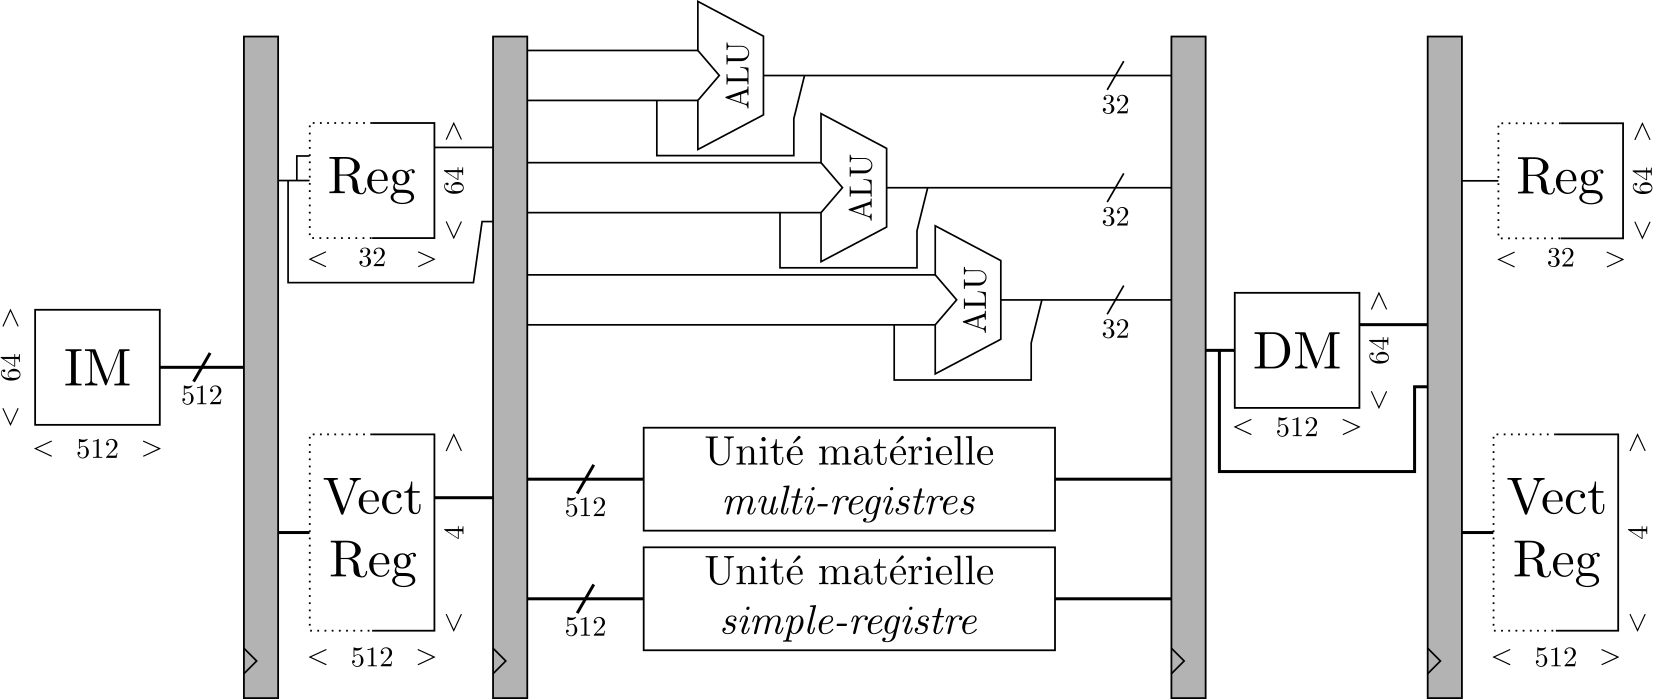
\includegraphics[width=\textwidth]{main/ch3_fig/full_tensilica}
\caption{Architecture de l'ASIP proposé.}
\label{fig:full_tensilica}
\end{figure}

Les instructions spécialisées réalisent des fonctions équivalentes à celles des PEs des architectures matérielles qui ont été présentées dans la sous-section \ref{subsec:hard_sc}. Il s'agit des fonctions $f$, $g$, \texttt{R1}, \texttt{R0}, \texttt{REP} et \texttt{SPC}. Deux types d'instructions spécialisées ont été conçus et ajoutés au processeur proposé comme montré dans \ref{fig:full_tensilica}. Les premières sont les instructions \textit{multi-registres} et les secondes les instructions \textit{simple-registre}. \'A l'image des PEs de l'architecture semi-parallèle, leur niveau de parallélisme est fixé ($P=64$). Une file de registres vectoriels permet de stocker des données sur 512 bits. Les instructions \textit{multi-registres} lisent et écrivent dans cette file de registres vectoriels.

Ces instructions spécialisées sont décrites à l'aide du langage TIE associé aux outils de Tensilica.
L'implémentation de la fonction $f$ est représentée dans la Figure~\ref{fig:f_tie}. Les deux opérandes sont les LLRs notés $L_a$ et $L_b$ et la sortie est notée $f(L_a,L_b)$. Ces deux entrées et la sortie correspondent à des registres de la file de registres vectoriels. Afin de clarifier le schéma, le niveau de parallélisme dans la Figure~\ref{fig:f_tie} a été réduit à $P=4$. Dans la plupart des décodeurs polaires, pour réduire le chemin critique, les LLRs sont représentés au format \og signe-amplitude \fg : un bit est utilisé pour le signe, et le reste pour la valeur absolue. En revanche, dans notre implémentation, les données sont représentées en complément à deux, car il s'agit du mode de représentation utilisé dans les processeurs XTensa.
L'architecture associée à la fonction $g$ est détaillée dans la Figure~\ref{fig:g_tie}. Cette fonction consiste en une addition simple avec une inversion de signe selon la valeur de la somme partielle $s_a$.
La fonction $h$ n'est pas représentée, il s'agit d'un simple \textit{ou-exclusif} entre les sommes partielles d'entrées. Les fonctions \texttt{R0} et \texttt{R1} sont également simples. La première consiste en une mise à zéro des sorties. La seconde est un seuillage des variables d'entrée. Le seuillage est une simple copie du bit de poids fort.
\begin{figure}[t]
  \centering
  \subfloat[Fonction $f$]{
  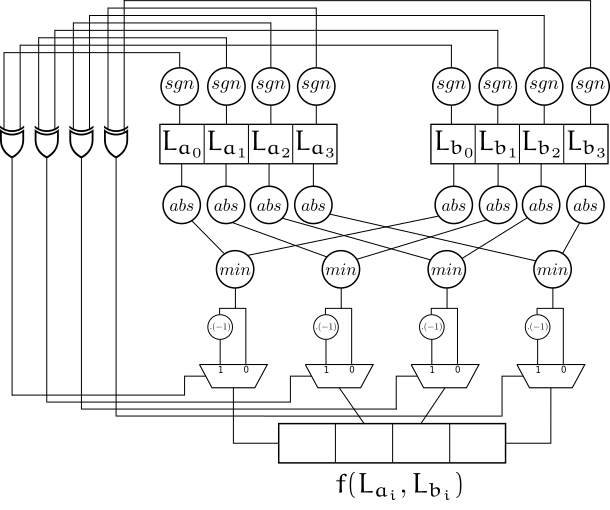
\includegraphics[scale=0.45]{main/ch3_fig/f_tie}
  \label{fig:f_tie}
  }
  \subfloat[Fonction $g$]{
  \includegraphics[scale=0.45]{main/ch3_fig/g_tie}
  \label{fig:g_tie}
  }
  \\\quad\quad\quad\quad\quad\quad
  \subfloat[Fonction \texttt{REP}]{
  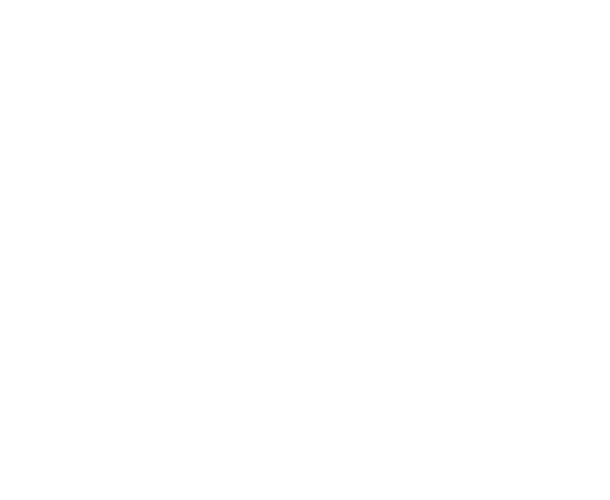
\includegraphics[scale=0.45]{main/ch3_fig/rep_tie}
  \label{fig:rep_tie}
  } \quad\quad\quad\quad\quad\quad\quad\quad\quad\quad
  \subfloat[Fonction \texttt{SPC}]{
  \includegraphics[scale=0.45]{main/ch3_fig/spc_tie}
  \label{fig:spc_tie}
  }
  \caption{Implémentations matérielles des instructions spécialisées.}
\end{figure}

Comme expliqué dans la sous-section~\ref{subsec:pruning}, le traitement d'un \noeud de répétition consiste en l'addition de tous les LLRs d'entrée pour former la variable notée \og \texttt{accum} \fg dans la Figure~\ref{fig:rep_tie}. Puis, une détection du signe de cette variable est effectuée. Elle détermine le vecteur $s$ en sortie. Un arbre binaire est parcouru afin de réaliser l'addition nécessaire. Pour éviter tout débordement, la taille du registre de stockage de la variable \texttt{accum} est de 32 bits.

L'unité matérielle de traitement des \noeuds \texttt{SPC} est représentée dans la Figure~\ref{fig:spc_tie}. Il s'agit de l'unité la plus complexe car elle comprend un tri des LLRs. Aussi, le parallélisme de cet unité est volontairement limité à 8 dans notre implémentation.

\subsection{Instructions spécialisées \textit{simple-registre}}

Dans les implémentations logicielles, la séquence d'opérations nécessaire à l'exécution des fonctions élémentaires polaires est la suivante : i) chargement depuis la mémoire cache vers les registres des variables d'entrée (LLRs et / ou sommes partielles), ii) calcul du résultat de la fonction élémentaire, en une ou plusieurs étapes, dont la sortie est stockée dans un registre, iii) sauvegarde de cette variable de sortie dans la mémoire cache du processeur.

Par ailleurs, dans les implémentations matérielles présentées dans la sous-section \ref{subsec:hard_sc}, le chemin de données part de la sortie de la mémoire, passe par les fonctions combinatoires réalisant les fonctions polaires élémentaires et finit à l'entrée de la mémoire. Ce chemin de données est parcouru en un seul cycle d'horloge. La méthode présentée dans cette sous-section, nommée \textit{simple-registre}, est conçue dans le but de reproduire le fonctionnement des implémentations matérielles de décodeur de codes polaires dans notre architecture de processeur.

\begin{figure}[t]
  \centering
  \subfloat[Unité matérielle \textit{simple-registre}.]{
  \includegraphics[scale=0.3]{main/ch3_fig/in_register_unit}
  \label{fig:in_register_unit}
  }\quad\quad\quad
  \subfloat[Un sous-arbre décodé grâce aux instructions \textit{simple-registre}.]{
  \includegraphics[scale=0.3]{main/ch3_fig/in_register_tree}
  \label{fig:in_register_tree}
  }
  \caption{Instructions \textit{simple-registre}.}
  \label{fig:simple-registre}
\end{figure}

La méthode \textit{simple-registre} est appliquée sur les sous-arbres de décodage dont le \noeud racine contient 64 LLRs. La Figure \ref{fig:in_register_tree} illustre un tel sous-arbre.
Ces 64 LLRs sont notés $\mathbold{L_{in}}$.
Lorsque le programme a généré les LLRs de la racine de ce sous-arbre, ceux-ci sont stockés dans un registre dédié.
Ce registre est noté $\mathbold{L}$ dans la Figure~\ref{fig:in_register_unit} qui décrit l'unité matérielle sur laquelle s'exécutent les instructions \textit{simple-registre}.
Le décodage du sous-arbre se fait ensuite intégralement à travers les registres, sans passer par la mémoire cache.
Les sommes partielles notées $\mathbold{s_{out}}$ constituent la sortie de l'unité matérielle.
Cette méthode reproduit le fonctionnement des implémentations matérielles de l'algorithme SC : l'exécution d'une fonction élémentaire quelconque, comprenant la lecture et l'écriture de la donnée depuis le registre, en un seul cycle d'horloge.

% \begin{figure}[htp]
% \centering
% 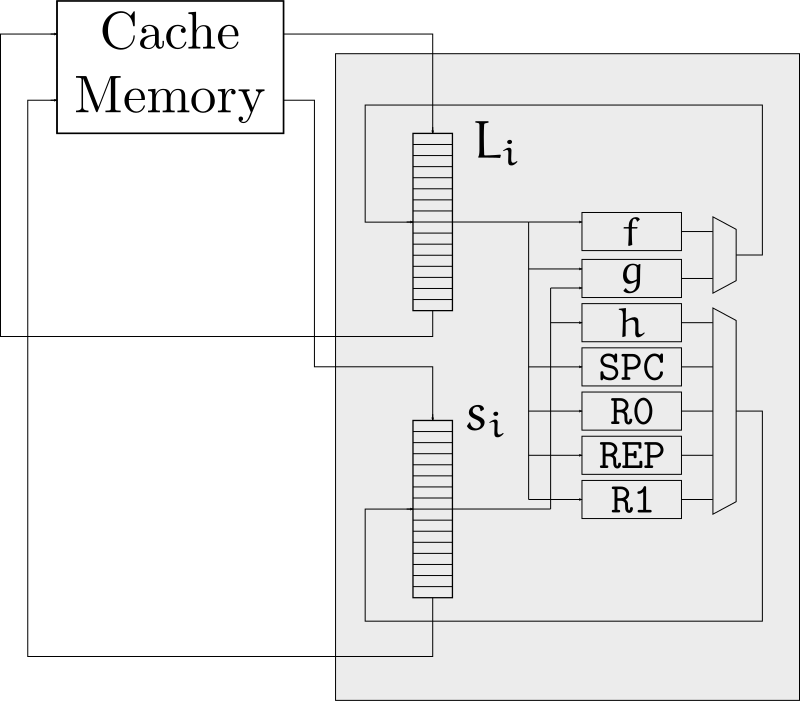
\includegraphics[width=0.7\textwidth]{main/ch3_fig/in_register}
% \caption{Instructions \textit{simple-registre}}
% \label{fig:simple-registre}
% \end{figure}




Elle résout également un problème récurrent des implémentations logicielles utilisant du parallélisme : l'alignement des données. En effet, pour pouvoir appliquer une fonction vectorielle des données de deux registres vectoriels, il est nécessaire de les aligner. Cela implique des opérations supplémentaires. Dans l'implémentation \textit{simple-registre}, l'alignement est prévu en amont et implémenté dans l'unité matérielle. Aucune instruction supplémentaire n'est nécessaire. 

\subsection{Description logicielle de l'algorithme de décodage}
\begin{figure}[t]
\lstset{language=C++,
        basicstyle=\footnotesize\ttfamily,
        keywordstyle=\bfseries\color{green!40!black},
        commentstyle=\itshape\color{purple!40!black},
        identifierstyle=\color{blue},
        stringstyle=\color{orange},
        morecomment=[l][\color{magenta}]{\#}
}
\begin{lstlisting}[language=C++, numbers=left, numbersep=0.3em, tabsize=2, basicstyle=\footnotesize\ttfamily]
inline void f_64(signed char* la, 
                 signed char* lb, 
                 signed char* lc)
{
  p512_a = (VR512*) la; // transtyper de char* vers VR512
  p512_b = (VR512*) lb; // transtyper de char* vers VR512
  p512_c = (VR512*) lc; // transtyper de char* vers VR512

  v512_a = *p512_a; // chargement des donnees vers VR512
  v512_b = *p512_b; // chargement des donnees vers VR512
  
  // execution de l'instruction specialisee
  v512_c = custom_f_64(v512_a, v512_b); 
  
  // sauvegarde du resultat en cache
  *p512_c = v512_c;     
}
\end{lstlisting}
\caption{Description logicielle de l'exécution d'une instruction spécialisée.}
\label{fig:f_code}
\end{figure}
L'ASIP ainsi proposé permet une l'exécution efficace de l'algorithme de décodage SC de codes polaires. Le décodage est décrit de manière logicielle, en langage C comprenant des instructions spécialisées. \`A titre d'information, un extrait du code source est donné dans la Figure~\ref{fig:f_code}. Tout d'abord, les fichiers d'en-tête produits par les outils de conception définissent les types associés aux files de registres vectoriels (\texttt{VR512}). Afin de charger une donnée en mémoire cache vers les registres vectoriels, il est nécessaire de créer des pointeurs vers ces variables de type (\texttt{VR512}). Les données sont ensuite chargées vers deux de ces registres vectoriels. La fonction spécialisée, ici la fonction \texttt{custom\_f\_64} est ensuite appliquée. Le résultat est stockée dans la mémoire cache.

Lors du développement, il est apparu qu'il était difficile de réduire la durée des opérations liées au parcours de l'arbre et aux tests associés. L'utilisation de l'option FLIX3 a permis une première réduction de ce temps, bien qu'insuffisante. La technique de déroulage présentée en sous-section~\ref{subsec:unroll} permet une réduction plus significative. Dérouler le code améliore la performance au prix d'une réduction de la flexibilité. Il faut en effet générer une version différente du code pour un ensemble donné de paramètres.


Dans l'implémentation logicielle proposée, une alternative au déroulage, nommée pseudo-déroulage, est privilégiée. Tout d'abord, toutes les fonctions élémentaires pour le décodage de codes polaires possèdent le même prototype de fonctions dans la description logicielle.
\begin{figure}[htp]
\lstset{language=C++,
        basicstyle=\footnotesize\ttfamily,
        keywordstyle=\bfseries\color{green!40!black},
        commentstyle=\itshape\color{purple!40!black},
        identifierstyle=\color{blue},
        stringstyle=\color{orange},
        morecomment=[l][\color{magenta}]{\#}
}
\begin{lstlisting}[language=C++, numbers=left, numbersep=0.3em, tabsize=2, basicstyle=\footnotesize\ttfamily]
// fonction polaire spécialisée
void u_f_64(struct polar_operation& op)
{
    for(int i = 0; i < op.n_elmts; i+=64)
      F_64(op.arg0 + i, op.arg1 + i, op.arg2 + i);
}

// fonction polaire générique
typedef void (*polar_func)(struct polar_operation&);

// structure passée en argument de la fonction générique
struct polar_operation
{
  polar_func   p_func; // pointeur vers la fonction polaire spécialisée 

  signed char* arg0; // les arguments des fonctions polaires spécialisées
  signed char* arg1; // ces arguments sont souvent des adresses
  signed char* arg2;
  signed char* arg3;

  int          n_elmts; // le nombre d'éléments traités en parallèle
  int          off_s; // un offset nécessaire pour l'accès aux PSs
};

// le tableau polar_op_vec est initialisé lors de la construction
// du décodeur il contient la séquence des "polar operation"
std::vector<struct polar_operation> polar_op_vec;

// boucle principale du décodage
virtual void decode()
{
  const int n_op = polar_op_vec.size();
  for (int i = 0; i < n_op; i++)
  {
    // chaque fonction du tableau "polar_op_vec" est appelée
    polar_op_vec[i].p_func(polar_op_vec[i]); 
  }
}
\end{lstlisting}
\caption{Description logicielle du pseudo-déroulage.}
\label{fig:tensilica_code}
\end{figure}

Le type de fonction à appliquer ($f$, $g$, $h$, \texttt{R0}, \texttt{R1}, \texttt{SPC}, \texttt{REP}) est un paramètre de la fonction, accompagné des adresses auxquelles accéder aux données à lire et écrire. De cette manière, il est possible de créer, un tableau contenant les pointeurs des fonctions à appeler. L'algorithme permettant de déterminer la séquence de fonctions à exécuter prend comme entrée le tableau de bits gelés correspondant au code polaire.

Comme ce tableau est généré par le processeur lors de l'exécution, la généricité du décodeur est donc conservée. Les paramètres $N$ et $K$ ainsi que les indices des bits gelés sont données en entrée du programme. Ainsi, le processeur s'adapte automatiquement. Comme cela est détaillé dans la section suivante, ce pseudo-déroulage permet une réduction significatives du nombre de cycles d'horloges nécessaires au décodage d'un mot de code.


\section{Expérimentations et mesures}
\label{sec:tensilica_res}
Afin d'évaluer le processeur conçu, des expérimentations ont été réalisées. Le but est d'une part de quantifier le gain associé aux différentes améliorations du processeur, d'autre part de comparer les performances de débit, de latence et de consommation énergétique de l'architecture proposée avec celles obtenues sur d'autres architectures programmables.
\subsection{Mesure du gain lié à la spécialisation du processeur.}

Les codes polaires considérés ont été construits selon le document spécifiant les techniques de modulation et de codage pour le futur standard 5G \cite{3gpp_ts_2017-1}. 
La version académique des outils de conception de Tensilica ne permettent pas d'effectuer une synthèse logique du processeur ou d'accéder à sa description RTL. Seules des estimations de la fréquence, de la consommation et de la surface occupée sont disponibles. Nous avons sélectionné la technologie HPM 28nm de TSMC pour ces estimations.

Le Tableau \ref{tab:evolution_tensilica} présente l'impact des améliorations principales apportées au processeur de base. Un code polaire (32768,29492) est décodé. Il s'agit là du code utilisé durant le développement du processeur. Les mémoires de données et d'instructions sont dimensionnées pour ce code. La première implémentation logicielle de l'algorithme SC sur l'architecture de base du processeur XTensa LX7 nécessite 7.3 millions de cycles d'exécution pour décoder un mot de code. Quant à l'architecture spécialisée pour le décodage de codes polaires combinée à la technique de pseudo-déroulage de la description logicielle, elle permet de réduire le nombre de cycles d'exécution d'un facteur 50. Les instructions \textit{multi-registres} sont responsables d'une grande partie de cette réduction. Elles permettent à elles seules de diminuer d'un ordre de grandeur le nombre de cycles nécessaire au décodage d'un mot de code.
 \begin{table}[htp]
    \renewcommand{\arraystretch}{1.1}
    \centering
    \caption{Impact de chaque amélioration de l'ASIP sur le nombre de cycles d'horloges nécessaires pour décoder une trame, le débit et la surface occupée. La taille des mémoires n'est pas prise en compte pour la surface occupée. Fréquence considérée : 835 MHz.}
    \label{tab:evolution_tensilica}
    {\small\resizebox{\linewidth}{!}{
    \begin{tabular}{l | c  c  c }
    \multirow{2}{*}{\textbf{Version du processeur}}       & \multirow{2}{*}{\textbf{\# cycles}}   & $\bm{\mathcal{T}_i}$  &   \textbf{Surface}          \\
                                                 &             &  \textbf{(Mb/s)}          &  \textbf{(portes)}          \\
    \cmidrule(lr){1-1}
    \cmidrule(lr){2-2}
    \cmidrule(lr){3-3}
    \cmidrule(lr){4-4}
Processeur de base                               &   $7.30\times10^6$  &   $3.4$            & $160000$             \\

+ instructions \textit{multi-registres} $f$,$g$ et $h$   &   $2.64\times10^6$  &   $9.3$            & $210500$             \\

+ instructions \textit{multi-registres} \texttt{R0},
\texttt{R1},\texttt{SPC} et \texttt{REP}         & $534.00\times10^3$  &   $ 46$            & $272000$             \\

+ FLIX3                                          & $296.00\times10^3$  &   $ 83$            & $311900$             \\

+ instructions \textit{simple-registre}              & $192.00\times10^3$  &   $128$            & $445500$             \\

+ pseudo unrolled                                & $151.00\times10^3$  &   $163$            & $445500$             \\
    \end{tabular}
    }}
  \end{table}


La puissance consommée estimée pour la version complète de l'ASIP est de 111 mW, et la surface occupée est 0.475 mm\textsuperscript{2}. La fréquence estimée est 835 MHz. Cependant, les instructions spécialisées ne sont pas prises en compte pour l'estimation de la fréquence. En conséquence, un scénario plus réaliste où la fréquence de fonctionnement est 400 MHz est également présentée. Pour cette fréquence, la consommation estimée est 49 mW et la surface occupée 0.374 mm\textsuperscript{2}.

\subsection{Comparaison avec un processeur ARM}

Le logiciel AFF3CT développé par l'équipe CSN du laboratoire IMS de Bordeaux est utilisé pour exécuter une implémentation optimisée de l'algorithme SC sur un processeur ARM Cortex A57. La méthode de parallélisation \textit{intra-trame} est utilisée, et les LLRs sont représentés sur 8 bits en virgule fixe. La taille des données gérées par les instructions NEON est de 128 bits. Cela signifie que le parallélisme est égal à 16. Les résultats ici reportés ont été fournis par les auteurs de \cite{cassagne_energy_2016}. Dans ces résultats, la consommation de la mémoire RAM n'est pas prise en compte.
Le nombre moyens de cycles d'horloges nécessaire à chaque processeur pour décoder une trame est donné dans la Figure~\ref{fig:cycle_count}. Le processeur proposé permet une réduction significative du nombre de cycles grâce à l'utilisation d'unités matérielles de calcul spécialisées. La courbe tracée représente le rapport entre les nombres de cycle d'horloge de chaque processeur. Ce rapport est d'autant plus grand que $N$ est faible. Ceci est dû au fait que lorsque $N$ est faible, ce sont les instructions \textit{simple-registre} qui sont le plus utilisées. Or ces instructions sont les plus efficaces.
Cependant, ce nombre réduit de cycles d'horloge est contrebalancé par une fréquence réduite comme montré dans le Tableau~\ref{tab:asip}. Néanmoins, même dans le scénario le plus pessimiste, avec une fréquence de 400 MHz, le débit atteint par le processeur proposé est similaire à celui obtenu avec le processeur ARM. Qui plus est, l'énergie dépensée par bit décodé est 10 fois inférieur pour l'ASIP.
\begin{figure}[htp]
\centering
\includegraphics{main/ch3_fig/curves/cycle_count/cycle_count}
\caption{Comparaison du nombre de cycles de l'horloge nécessaires au décodage SC entre le Cortex ARM A57 et l'ASIP proposé.}
\label{fig:cycle_count}
\end{figure}

\subsection{Comparaison avec un processeur d'architecture x86}
Les débits, latences et l'énergie consommée par bit du décodeur logiciel SC inclus dans le logiciel AFF3CT ont également été mesurés sur un processeur Intel i7-4712HQ.
La puissance du \coeur est évaluée avec l'outil \texttt{powergadget} d'Intel. Seule la consommation du \coeur du processeur, excluant la consommation de la mémoire cache de niveau 3 et de la mémoire externe, est reportée. Cette fois-ci, le niveau de parallélisme est de 32. Ce niveau est atteint à l'aide du jeu d'instructions AVX2. La fréquence du CPU mesurée durant l'exécution est de 3.3 GHz. Les résultats récapitulés dans le Tableau \ref{tab:asip} montrent que le débit et la latence des implémentations de décodeur SC sur les processeurs i7 sont bien meilleurs que ceux obtenus avec le processeur ASIP proposé ou avec le processeur ARM. Cependant, la consommation énergétique est moins bonne. Une implémentation \textit{inter-trame} permettrait d'augmenter cette efficacité énergétique, au prix d'une augmentation de la latence, comme démontré dans \cite{cassagne_energy_2016}.


\begin{table}[htp]
  \centering
  \caption{Comparaison de la latence, du débit et de la consommation énergétique de décodeurs SC pour différents processeurs.}
  \label{tab:asip}
%\scriptsize
  \begin{tabular}{ccccc}
    \toprule

    Target & $N$ & \begin{tabular}{c}Latency\\{[$\mu$s]}\end{tabular} & \begin{tabular}{c}Throughput\\{[Mb/s]}\end{tabular} & \begin{tabular}{c}$E_b$\\{[nJ]}\end{tabular} \\

    \cmidrule(lr){1-1}
    \cmidrule(lr){2-2}
    \cmidrule(lr){3-5}

    \multirow{4}{*}{\bf A57-1.1GHz}
     & $1024$  & $13$  & $38$  & $21$  \\
     & $512$   & $6.7$ & $38$  & $21$  \\
     & $256$   & $3.6$ & $35$  & $22$  \\
     & $128$   & $2.1$ & $30$  & $27$  \\
    \midrule
    \multirow{4}{*}{\bf i7-3.3GHz}
     & $1024$  & $2.3$ & $222$ & $47$  \\
     & $512$   & $1.4$ & $182$ & $57$  \\
     & $256$   & $0.8$ & $155$ & $68$  \\
     & $128$   & $0.5$ & $124$ & $85$  \\
    \midrule
    \multirow{4}{*}{\bf ASIP-835MHz}
     & $1024$  & $7.2$ & $71$  & $1.6$ \\
     & $512$   & $3.9$ & $66$  & $1.7$ \\
     & $256$   & $1.9$ & $65$  & $1.7$ \\
     & $128$   & $1.0$ & $62$  & $1.8$ \\
    \midrule
    \multirow{4}{*}{\bf ASIP-400MHz}
     & $1024$  & $15$ &  $34$  & $1.4$ \\
     & $512$   & $8.2$ & $31$  & $1.6$ \\
     & $256$   & $4.1$ & $31$  & $1.6$ \\
     & $128$   & $2.1$ & $30$  & $1.7$ \\
    \bottomrule
  \end{tabular}
\end{table}

\section*{Conclusion}

Une première architecture de processeur ASIP spécialisée dans le décodage de codes polaires est présentée dans ce chapitre. Les outils logiciels de Tensilica permettent de spécialiser un processeur de type RISC. Après avoir détaillé la structure générale de ces microarchitectures RISC, nous expliquons comment elles peuvent être configurées et étendues par l'utilisation des outils logiciels de Tensilica. Les avantages et les enjeux liés à l'utilisation de tels outils de conception sont mis en avant.

Dans la deuxième partie du chapitre, nous expliquons comment ces outils ont été mis en œuvre pour notre problématique : le décodage de codes polaires. Tout d'abord les paramètres de l'architecture RISC de base sont modifiés et adaptés. Entre autres, une fonctionnalité permettant le support d'un parallélisme d'instruction est activée. La largeur du bus d'interface avec la mémoire de données est augmentée. Ensuite, des unités matérielles dédiées associées à des instructions spécialisées qui étendent le jeu d'instructions de base sont ajoutées. Enfin, une méthode de description logicielle nommée \og pseudo-déroulage \fg est proposé afin d'améliorer les performances de débit et de latence du processeur spécialisé conçu.

Dans une troisième partie, nous présentons et comparons le débit, la latence et la consommation du décodeur de type ASIP proposé avec les implémentations logicielles de codes polaires de l'état de l'art. Pour un code polaire (1024,512) décodé à l'aide de l'algorithme SC, le débit atteint est d'environ 70 Mb/s, dépassant les performances obtenues avec un processeur du marché de l'électronique embarquée. La consommation énergétique par rapport à ce même processeur est elle réduite d'un ordre de grandeur.
Cette contribution a été valorisée à travers une publication scientifique dans le cadre de la conférence ISCAS \cite{leonardon_custom_2018}.

Bien que ces résultats soient prometteurs, plusieurs limites concernant l'utilisation des outils et de la méthodologie de conception des processeurs XTensa ont été identifiés. Tout d'abord, le fait de ne pas disposer d'une licence complète empêche la génération du modèle matériel du processeur. Il est donc impossible de générer des résultats exhaustifs de synthèse et d'implémentation. Pour cette raison, les résultats obtenus sont des estimations fournies par l'outil, avec une marge d'erreur importante. De plus, le langage de descriptions matériel est le langage TIE, spécifique à la suite logicielle de Tensilica. Ceci limite les possibilités de réutilisation des unités matérielles conçues. D'autre part, une analyse attentive du code assembleur généré et des résultats de simulations montrent qu'une part significative de la durée d'exécution est prise par les échanges de données entre la mémoire cache, les registres et les unités matérielles de calcul. La conception et l'ajout des instructions \textit{simple-registre} permettent de diminuer le nombre de ces échanges. Mais cette amélioration est partielle et ne peut pas être appliquée sur l'ensemble de l'arbre de décodage.

Plusieurs outils alternatifs de conception d'ASIP ont été envisagés afin de résoudre ces problèmes. Parmi eux, la famille d'architectures \og TTA \fg a été sélectionnée pour créer le processeur présenté dans le chapitre suivant. Une des raisons de ce choix est la possibilité de contourner les registres et d'échanger les données directement entre la mémoire de données et les unités matérielles.             % Troisième thème (Doctorat) ou effacez ce fichier si vous êtes à la Maîtrise.
%!TEX root = ../my_thesis.tex
\chapter{Décodeurs polaires déclenchés par transport} % (fold)
\label{chap:tta}

\vspace*{\fill}
\minitocTITI
\vspace*{\fill}
\newpage

\section*{Introduction}



\section{Transport Triggered Architectures}
Au cours de ce manuscrit, du point de vue de l'architecture des processeurs, deux types de parallélisme ont été abordés.
Le premier est le parallélisme de données.
Pour exploiter ce parallélisme, les jeux d'instructions de certains processeurs incluent des instructions vectorielles SIMD.
C'est le cas des architectures ARM ou x86 actuelles qui incluent respectivement les jeux d'instructions NEON et AVX utilisés dans le Chapitre \ref{chap:soft_scl}.
Les instructions spécialisées de l'ASIP proposé dans le Chapitre \ref{chap:tensilica} sont également des instructions SIMD.
Ces instructions permettent d'appliquer parallèlement une même opération sur plusieurs données.

Le second type de parallélisme est le parallélisme d'instructions. Contrairement au parallélisme de données, il s'agit d'exécuter plusieurs opérations différentes sur plusieurs données d'entrées. Par exemple, effectuer une somme de deux données et, en parallèle, effectuer une opération \textit{ou-exclusif} sur deux autres.
Il existe plusieurs façons de concevoir un processeur permettant du parallélisme d'instructions. Le compilateur peut selon les cas être impliqué dans la détection et l'exploitation du parallélisme d'instructions.

Dans les architecture superscalaires, le compilateur n'est pas impliqué dans la gestion du parallélisme d'instructions. Celui-ci est détecté par des unités matérielles spécialisées. 
Elles permettent de lancer l'exécution de plusieurs opérations parallèles sur les multiples unités fonctionnelles du processeur.
Pour cela, ces unités ont la capacité d'analyser les dépendances entre les données, de changer dynamiquement l'ordre d'exécution des instructions, ainsi que de spéculer sur les futures instructions du programme exécuté. 
Un des avantages de ce type de processeurs est que des programmes séquentiels d'architectures plus anciennes peuvent être accélérés dans nouvelle compilation. Le désavantage est le complexité accrue du processeur causée par l'ajout des unités matérielles responsables de la mise en œuvre du parallélisme. La surface du circuit augmente ainsi que sa consommation énergétique.

Au contraire, dans les architectures dites \og à très long mot d'instruction \fg (VLIW : Very Large Instruction Word), l'essentiel de l'effort nécessaire à la mise en œuvre du parallélisme d'instructions est pris en charge par le compilateur. Le compilateur décrit quelles instructions doivent être exécutées en parallèle, et dans quel ordre. L'avantage des architectures VLIW par rapport aux architectures superscalaires est la réduction de la complexité de la logique de contrôle. De plus, les possibilité de parallélisme d'instructions sont plus facilement identifiées par les compilateurs qui ont une vue plus large du programme que les unités matérielles de parallélisation des architectures superscalaires.

L'architecture du processeur proposé dans ce chapitre fait partie de la famille des architectures déclenchées par le transport (TTA : Transport Triggered Architecture). Les TTAs sont des architectures modulaires particulières proches des architectures VLIW. La principale différences entre les architectures TTA et les architectures VLIW 



\subsection{Principes}


\begin{figure}
\centering
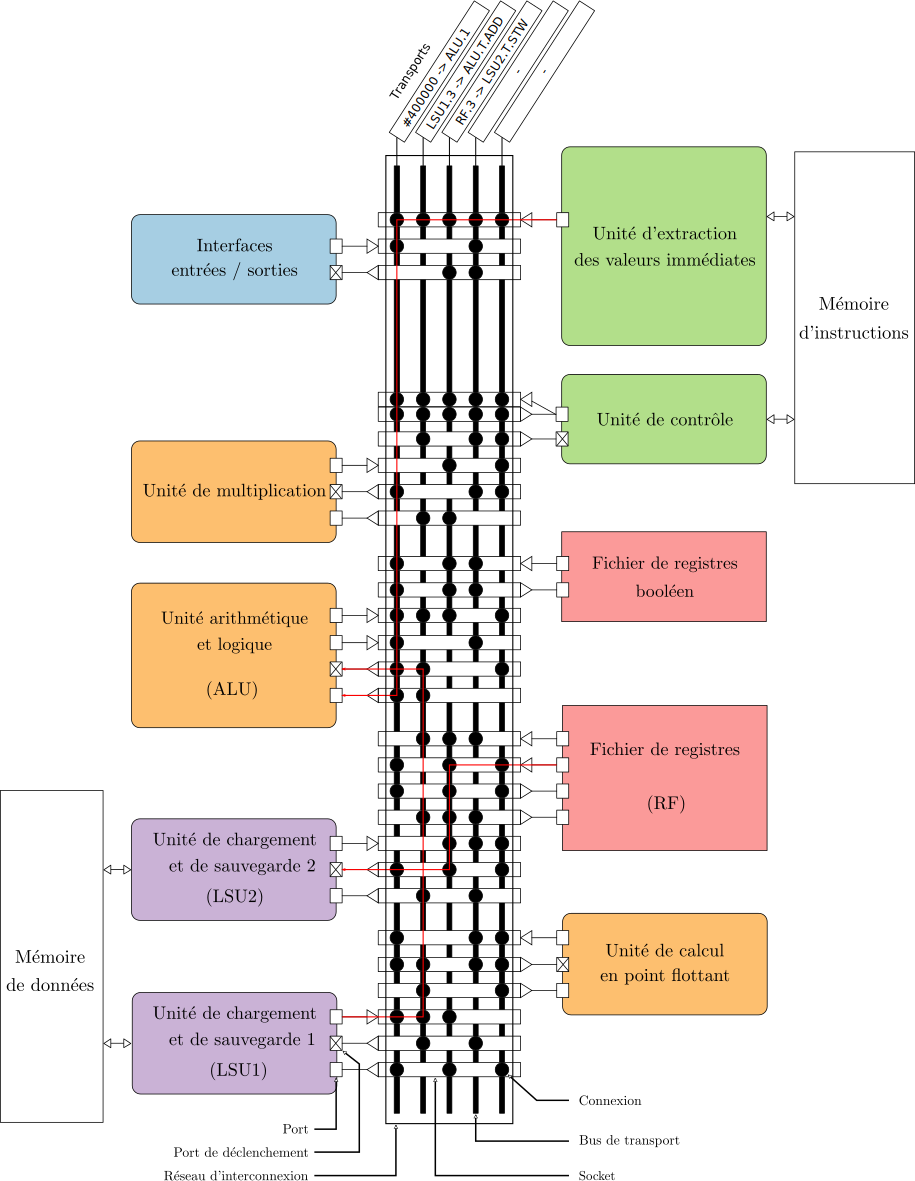
\includegraphics[width=\textwidth]{main/ch4_fig/archi_tta}
\caption{Un exemple d'architecture de processeur TTA. }
\end{figure}
\subsection{Environnement TCE}

\section{Transport Triggered Polar Decoders}

\subsection{Architecture du décodeur SC}
\subsection{Description logicielle}
\subsection{Implémentation de l'algorithme SCAN}

\section{Un flot de conception complet}

\subsection{Génération des vecteurs de tests}
\subsection{Cycles de conception}

\section{Expérimentations et mesures}

\subsection{TT-SC}
\subsection{TT-SCAN}


\section*{Conclusion}


             % Troisième thème (Doctorat) ou effacez ce fichier si vous êtes à la Maîtrise.
%!TEX root = ../my_thesis.tex
\chapter*{Conclusions et perspectives}
\markboth{Conclusions et perspectives}{Conclusions et perspectives}
\addcontentsline{toc}{chapter}{Conclusions et perspectives}
\section*{Conclusions}
\section*{Perspectives}
         % Conclusion.
%\backmatter
\ifthenelse{\equal{\Langue}{english}}{
	\renewcommand\bibname{BIBLIOGRAPHY}
	\bibliography{tail/bibliography}
	\bibliographystyle{IEEEtran}			% Bibliography style.
}{
	\renewcommand\bibname{RÉFÉRENCES}
	\bibliography{tail/bibliography}
	\bibliographystyle{IEEEtran-francais}    % Style de la bibliographie.
	\bibliographystylemine{IEEEtran-francais}
	\bibliographymine{tail/bibliography}
}
%
\ifthenelse{\equal{\AnnexesPresentes}{O}}{
	\appendix%
	\newcommand{\Annexe}[1]{\annexe{#1}\setcounter{figure}{0}\setcounter{table}{0}\setcounter{footnote}{0}}%
	%!TEX root = ../my_thesis.tex

\appendix

\chapter{Compléments au Chapitre 1}
\section{Détails 1}\label{append:decoding_nodes}

Les sorties du canal composite sont des informations souples données par le démodulateur.
Ce bruit additif est ajouté à la valeur des données en sortie du modulateur $\mathbold{x}$.
\begin{equation}
y_i = x_i + n_i
\end{equation}
Dans le modèle de chaine de communication considéré, la puissance du bruit du canal AWGN $N_0$ est supposée connue.
Cela permet au démodulateur de calculer la probabilité conditionnelle suivante.
\begin{equation}
	P_r( \tilde{y}_i|\tilde{x}_i) = \dfrac{1}{\sqrt{\pi N_0}}\exp^{-\tfrac{(\tilde{x}_i^2-\tilde{y}_i^2)}{N_0}}
\end{equation}
$p_i$ représente la probabilité de recevoir $\tilde{y}_i$ en présupposant la valeur de $\tilde{x}_i$ en sortie du modulateur ($\tilde{x}_i=-1$ ou $\tilde{x}_i=1$). Les \textit{likelihood ratios} (LRs), sont exprimés en fonction de ces probabilités :
\begin{equation}
	l_i = \log\left(\dfrac{P_r(y_i | x_i = 0)}{P_r(y_i | x_i = 1)}\right)
\end{equation}
\label{eq:lr}

Les \textit{log likelihood ratios} (LLR), sont le logarithme népérien des LR ! 

\begin{equation}
  L_i = \log\left(\dfrac{P_r(y_i | x_i = 0)}{P_r(y_i | x_i = 1)}\right)
\end{equation}
\label{eq:llr}


Les codes correcteurs d'erreurs peuvent être définis par un ensemble de contraintes de parités. Une représentation graphique de ces contraintes est appelé \textit{graphe de Tanner} comme représenté en Figure~\ref{fig:noeuds}.

\begin{figure}[t]
\centering
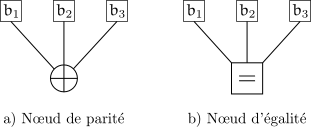
\includegraphics{tail/appendix_1_fig/noeuds}
\caption{Représentations des noeuds de décodage}
\label{fig:noeuds}
\end{figure}

Le noeud de parité est la représentation graphique de l'équation suivante : 
\begin{equation}
b_0 + b_1 + b_2 = 0
\end{equation}
Tandis que l'encodeur canal associe le vecteur d'entrée $\mathbold{b}$ de longueur $K$ à un mot de code $\mathbold{x}$ de longueur $N$, le décodeur combine les différents LR ou LLR en sortie du canal composite dans le but de retrouver les bits d'origine.
Dans l'exemple de la Figure~\ref{fig:noeuds}, les estimations du canal pour les valeurs des bits $b_1$ et $b_2$, notés respectivement $l_1$ et $l_2$, peuvent être combinées afin de calculer une estimation extrinsèque du bit $b_0$, notée $l_0^e$.

Sa valeur est par définition :
\begin{equation}
l^e_0 = \dfrac{P(y_1,y_2 | b_0 = 0)}{P(y_1,y_2 | b_0 = 1)}
\label{eq:le0}
\end{equation}
Seules deux combinaisons possibles des bits $b_1$ et $b_2$ peuvent impliquer que $b_0$ soit égal à $0$ : ou bien $b_1=0$ et $b_2=0$, ou bien $b_1=1$ et $b_2=1$. Il est donc possible de calculer $P(b_0|y_1,y_2)$ : 
\begin{equation}
P(y_1,y_2 | b_0 = 0)  =  P(y_1 | b_1 = 0)P(y_2 | b_2 = 0) + P(y_1 | b_1 = 1)P(y_2 | b_2 = 1) \\
\end{equation}
Donc,  
\begin{equation}
P(y_1,y_2 | b_0 = 0)  =  l_1l_2 + 1 \\
\label{eq:le1}
\end{equation}


De la même manière,
\begin{equation}
P(b_0 = 1 | y_1,y_2) =P(y_1 | b_1 = 0)P(y_2 | b_2 = 1) + P(y_1 | b_1 = 1)P(y_2 | b_2 = 0)
\end{equation}
Donc, 
\begin{equation}
P(b_0 = 1 | y_1,y_2) = l_1 + l_2
\label{eq:le2}
\end{equation}
On déduit donc de \ref{eq:le0}, \ref{eq:le1} et \ref{eq:le2} : 

\begin{equation}
l^e_0=\dfrac{1 + l_1l_2}{l_1+l_2}
\label{eq:parity}
\end{equation}

En effectuant la même démarche pour le N\oe{}ud d'égalité il est possible d'obtenir :
\begin{eqnarray*}
\begin{array}{r c l}
P(y_1,y_2|b_0=0) & = & P(y_1|b_1=0) P(y_2 | b_2 = 0) \\
P(y_1,y_2|b_0=1) & = & P(y_1|b_1=1) P(y_2 | b_2 = 1) 
\end{array}
\end{eqnarray*}
Il est possible d'en déduire l'extrinsèque :
\begin{equation}
l^e_0=l_1l_2
\label{eq:equality}
\end{equation}

L'algorithme de décodage SC peut être représenté sous la forme de \textit{factor graph} dans lequel les équations \ref{eq:parity} et \ref{eq:equality} sont appliquées, comme montré en Figure~\ref{fig:SCSchedule}. Les fonctions élémentaires F et G sont des combinaisons des équations liées aux \noeuds de parité et aux \noeuds d'égalités.
\begin{figure}[t]
  \centering
  \subfloat[][$F$ function]{\includegraphics[width=.24\textwidth]{tail/appendix_1_fig/SC_graph2_b}}\quad\quad\quad\quad
  \subfloat[][$G$ function]{\includegraphics[width=.25\textwidth]{tail/appendix_1_fig/SC_graph2_d}}
  \caption{Fonctions $F$ et $G$ de l'algorithme SC}
  \label{fig:SCSchedule}
\end{figure}
\begin{equation}
l_{0,0} = F(l_{0,1}, l_{1,1}) = \dfrac{1+l_{0,1}l_{1,1}}{l_{0,1}+l_{1,1}}
\end{equation}
\[
	l_{1,0} = 
	\begin{cases} 
	l_{1,1}l_{0,1} & \text{if }S_{0,0} = 0\\
	l_{1,1}\dfrac{1}{l_{0,1}} & \text{if }S_{0,0} = 1
	\end{cases}
\]
Cela peut être simplifié : 
\begin{equation}
l_{1,0} = G(l_{1,1},l_{0,1},S_{0,0}) = l_{1,1}l_{0,1}^{1 - 2S_{0,0}}
\end{equation}

Ces équations utilisent des LR. Elles peuvent être modifiées afin de faire apparaître les LLR : 

\begin{equation}
L_{0,0} = f(L_{0,1}, L_{1,1}) = 2\tanh^{-1}(\tanh(L_{0,1})\tanh(L_{1,1}))
\end{equation}
\begin{equation}
L_{1,0} = g(L_{1,1},L_{0,1},S_{0,0}) = L_{1,1} + (1 - 2S_{0,0})L_{0,1}
\end{equation}

Enfin, $f$ peut être simplifiée \cite{fossorier1999reduced} : 
\begin{equation}
f(L_{0,1}, L_{1,1}) \approx \text{sign}(L_{0,1})\text{sign}(L_{1,1})\text{min}(|L_{0,1}|,|L_{1,1}|))
\end{equation}}
{}
\end{document}
